\documentclass[titlepage=true]{scrartcl}

%%%%%%%%%%%%%%%%%%%%%%%%%%%%%%%%%%%%%%%
%% Makros & anderer Low-Level bastel %%
%%%%%%%%%%%%%%%%%%%%%%%%%%%%%%%%%%%%%%%
\makeatletter
%% Makros für Titel, Autor und Datum 
%% Dank diesem Makro stehen Titel, Autor und Datum überall im Dokument zur verfügung
%% Date hat zudem den Default-Wert \today
\def\@Title{}
\def\@Author{}
\def\@Date{\today}
\newcommand{\Title}{\@Title}
\newcommand{\Author}{\@Author}
\newcommand{\Date}{\@Date}
\AtBeginDocument{%
  \let\@Title\@title
  \let\@Author\@author
  \let\@Date\@date
}

%% Makros für den Arraystretch (bei uns meist in Tabellen genutzt, welche Formeln enthalten)
% Default Value
\def\@ArrayStretchDefault{1} % Entspricht der Voreinstellung von Latex

% Setzt einen neuen Wert für den arraystretch
\newcommand{\setArrayStretch}[1]{\renewcommand{\arraystretch}{#1}}

% Setzt den arraystretch zurück auf den default wert
\newcommand{\resetArrayStretch}{\renewcommand{\arraystretch}{\@ArrayStretchDefault}}

% Makro zum setzten des Default arraystretch. Kann nur in der Präambel verwendet werden.
\newcommand{\setDefaultArrayStretch}[1]{%
	\AtBeginDocument{%
		\def\@ArrayStretchDefault{#1}
		\renewcommand{\arraystretch}{#1}
	}
}
\makeatother


%%%%%%%%%%%%%%%%%%%%%%%
%% Wichtige Packages %%
%%%%%%%%%%%%%%%%%%%%%%%
\usepackage[utf8]{inputenc} % UTF-8 unterstützung
\usepackage[english, ngerman]{babel} % Silbentrennung
%\usepackage[automark]{scrpage2} % Header und Footer
\usepackage[automark]{scrlayer-scrpage} % Header und Footer
\usepackage{tabularx}

% Für Abbildungen mit mehreren kleinen Bilder
% Doku: http://www.ctan.org/tex-archive/macros/latex/contrib/caption/
\usepackage{caption}
\usepackage{subcaption}

% Für die Nutzung von "tabular" (Tabulator)
\usepackage{listliketab}
\usepackage{placeins}
\ifx \GUARDhsrColors \undefined
\def\GUARDhsrColors{}

\usepackage[table]{xcolor}

\definecolor{HSRWhite}{cmyk}{0,0,0,0}

\definecolor{HSRBlue}{cmyk}{1,0.4,0,0.2}
\definecolor{HSRBlue80}{cmyk}{0.8,0.32,0,0.16}
\definecolor{HSRBlue60}{cmyk}{0.6,0.24,0,0.12}
\definecolor{HSRBlue40}{cmyk}{0.4,0.16,0,0.08}
\definecolor{HSRBlue20}{cmyk}{0.2,0.08,0,0.04}

\definecolor{HSRLightGray}{cmyk}{0,0,0,0.30}
\definecolor{HSRLightGray80}{cmyk}{0,0,0,0.24}
\definecolor{HSRLightGray60}{cmyk}{0,0,0,0.18}
\definecolor{HSRLightGray40}{cmyk}{0,0,0,0.12}
\definecolor{HSRLightGray20}{cmyk}{0,0,0,0.06}

\definecolor{HSRSchwarz}{cmyk}{0,0,0,1}
\definecolor{HSRSchwarz80}{cmyk}{0,0,0,0.8}
\definecolor{HSRSchwarz60}{cmyk}{0,0,0,0.6}
\definecolor{HSRSchwarz40}{cmyk}{0,0,0,0.4}
\definecolor{HSRSchwarz20}{cmyk}{0,0,0,0.2}

\definecolor{HSRHematite}{cmyk}{0.6,1,0.4,0.2}
\definecolor{HSRHematite80}{cmyk}{0.48,0.80,0.32,0.16}
\definecolor{HSRHematite60}{cmyk}{0.36,0.60,0.24,0.12}
\definecolor{HSRHematite40}{cmyk}{0.24,0.40,0.16,0.08}
\definecolor{HSRHematite20}{cmyk}{0.12,0.20,0.08,0.04}

\definecolor{HSRLakeGreen}{cmyk}{0.70,0.30,0.45,0.05}
\definecolor{HSRLakeGreen80}{cmyk}{0.56,0.24,0.36,0.03}
\definecolor{HSRLakeGreen60}{cmyk}{0.42,0.18,0.27,0.02}
\definecolor{HSRLakeGreen40}{cmyk}{0.28,0.06,0.13,0.06}
\definecolor{HSRLakeGreen20}{cmyk}{0.14,0.06,0.09,0.01}

\definecolor{HSRReed}{cmyk}{0.10,0.25,0.45,0.60}
\definecolor{HSRReed80}{cmyk}{0.08,0.20,0.36,0.48}
\definecolor{HSRReed60}{cmyk}{0.06,0.15,0.27,0.36}
\definecolor{HSRReed40}{cmyk}{0.04,0.10,0.18,0.24}
\definecolor{HSRReed20}{cmyk}{0.02,0.05,0.09,0.12}

\definecolor{HSRPetrol}{cmyk}{1,0.18,0,0.45}
\definecolor{HSRPetrol80}{cmyk}{0.64,0.08,0.12,0.32}
\definecolor{HSRPetrol60}{cmyk}{0.48,0.06,0.09,0.24}
\definecolor{HSRPetrol40}{cmyk}{0.32,0.04,0.06,0.16}
\definecolor{HSRPetrol20}{cmyk}{0.16,0.02,0.03,0.08}

\definecolor{HSRBasswood}{cmyk}{0.25,0.05,0.70,0.15}
\definecolor{HSRBasswood80}{cmyk}{0.20,0.04,0.56,0.12}
\definecolor{HSRBasswood60}{cmyk}{0.15,0.03,0.42,0.09}
\definecolor{HSRBasswood40}{cmyk}{0.10,0.02,0.28,0.06}
\definecolor{HSRBasswood20}{cmyk}{0.05,0.01,0.14,0.03}


\fi
\ifx\GUARDmathe\undefined
\def\GUARDmathe{}

\usepackage{amssymb}
% Das mathtools package ist eine Erweiterung zum amsmath package.
% Das amsmath package wird dabei automatisch geladen
\usepackage{mathtools}


% Package mit vielen weiteren Mathe Symbolen
% http://www.ctan.org/tex-archive/fonts/mathabx
\usepackage{mathabx}

\fi
\ifx\GUARDenumitem\undefined
\def\GUARDenumitem{}

\usepackage{enumitem}

\fi

% Seitenränder für Formelsammlungen
\usepackage[left=1cm,right=1cm,top=1cm,bottom=1cm,includeheadfoot,headsep=0.2cm,footskip = \dimexpr\headsep+\ht\strutbox\relax]{geometry}

\usepackage{multirow} % Create tabular cells spanning multiple rows
\usepackage{multicol} % In­ter­mix sin­gle and mul­ti­ple columns
\usepackage{rotating} % Rotation tools, including rotated fullpage floats


%%%%%%%%%%%%%%%%%%%%%%%%%%%%%%%%%%%
%% Layout der Kopf und Fusszeile %%
%%%%%%%%%%%%%%%%%%%%%%%%%%%%%%%%%%%
\deftripstyle{zusammenfassung}[0pt][0.5pt]
	{\Title}	% Kopfzeile innen
	{\headmark}	% Kopfzeile mitte
	{\pagemark}	% Kopfzeile aussen
	{\Author}	% Fusszeile innen
	{
\includegraphics[width=1.6cm]{./header/lizenzen/cc-by-nc-sa/small.png}}			% Fusszeile mitte
	{\Date}	% Fusszeile aussen
\pagestyle{zusammenfassung}



% Makros für Verweise auf ein Buch oder Skript
\newcommand{\buch}[1]{$_{\textcolor{HSRLakeGreen}{\mbox{\small{#1}}}}$}
\newcommand{\skript}[1]{$_{\textcolor{HSRReed}{\mbox{\small{#1}}}}$}

\setlength{\parindent}{0pt}
\ifx\GUARDhyperref\undefined
\def\GUARDhyperref{}

\ifx \GUARDhsrColors \undefined
\def\GUARDhsrColors{}

\usepackage[table]{xcolor}

\definecolor{HSRWhite}{cmyk}{0,0,0,0}

\definecolor{HSRBlue}{cmyk}{1,0.4,0,0.2}
\definecolor{HSRBlue80}{cmyk}{0.8,0.32,0,0.16}
\definecolor{HSRBlue60}{cmyk}{0.6,0.24,0,0.12}
\definecolor{HSRBlue40}{cmyk}{0.4,0.16,0,0.08}
\definecolor{HSRBlue20}{cmyk}{0.2,0.08,0,0.04}

\definecolor{HSRLightGray}{cmyk}{0,0,0,0.30}
\definecolor{HSRLightGray80}{cmyk}{0,0,0,0.24}
\definecolor{HSRLightGray60}{cmyk}{0,0,0,0.18}
\definecolor{HSRLightGray40}{cmyk}{0,0,0,0.12}
\definecolor{HSRLightGray20}{cmyk}{0,0,0,0.06}

\definecolor{HSRSchwarz}{cmyk}{0,0,0,1}
\definecolor{HSRSchwarz80}{cmyk}{0,0,0,0.8}
\definecolor{HSRSchwarz60}{cmyk}{0,0,0,0.6}
\definecolor{HSRSchwarz40}{cmyk}{0,0,0,0.4}
\definecolor{HSRSchwarz20}{cmyk}{0,0,0,0.2}

\definecolor{HSRHematite}{cmyk}{0.6,1,0.4,0.2}
\definecolor{HSRHematite80}{cmyk}{0.48,0.80,0.32,0.16}
\definecolor{HSRHematite60}{cmyk}{0.36,0.60,0.24,0.12}
\definecolor{HSRHematite40}{cmyk}{0.24,0.40,0.16,0.08}
\definecolor{HSRHematite20}{cmyk}{0.12,0.20,0.08,0.04}

\definecolor{HSRLakeGreen}{cmyk}{0.70,0.30,0.45,0.05}
\definecolor{HSRLakeGreen80}{cmyk}{0.56,0.24,0.36,0.03}
\definecolor{HSRLakeGreen60}{cmyk}{0.42,0.18,0.27,0.02}
\definecolor{HSRLakeGreen40}{cmyk}{0.28,0.06,0.13,0.06}
\definecolor{HSRLakeGreen20}{cmyk}{0.14,0.06,0.09,0.01}

\definecolor{HSRReed}{cmyk}{0.10,0.25,0.45,0.60}
\definecolor{HSRReed80}{cmyk}{0.08,0.20,0.36,0.48}
\definecolor{HSRReed60}{cmyk}{0.06,0.15,0.27,0.36}
\definecolor{HSRReed40}{cmyk}{0.04,0.10,0.18,0.24}
\definecolor{HSRReed20}{cmyk}{0.02,0.05,0.09,0.12}

\definecolor{HSRPetrol}{cmyk}{1,0.18,0,0.45}
\definecolor{HSRPetrol80}{cmyk}{0.64,0.08,0.12,0.32}
\definecolor{HSRPetrol60}{cmyk}{0.48,0.06,0.09,0.24}
\definecolor{HSRPetrol40}{cmyk}{0.32,0.04,0.06,0.16}
\definecolor{HSRPetrol20}{cmyk}{0.16,0.02,0.03,0.08}

\definecolor{HSRBasswood}{cmyk}{0.25,0.05,0.70,0.15}
\definecolor{HSRBasswood80}{cmyk}{0.20,0.04,0.56,0.12}
\definecolor{HSRBasswood60}{cmyk}{0.15,0.03,0.42,0.09}
\definecolor{HSRBasswood40}{cmyk}{0.10,0.02,0.28,0.06}
\definecolor{HSRBasswood20}{cmyk}{0.05,0.01,0.14,0.03}


\fi

\usepackage[plainpages=false,pdfpagelabels]{hyperref}
\hypersetup{
  pdfstartview={FitH}, % fits the width of the page to the window
  pdfauthor={\Author},
  pdfcreator={\Author},
  pdfproducer={\Author},
  pdftitle={\Title},
  colorlinks=true,
  linkcolor=HSRBlue,
  citecolor=HSRReed,
  filecolor=HSRLake,
  urlcolor=HSRHematite
}

\fi

\ifx\GUARDlistings\undefined
\def\GUARDlistings{}

\usepackage{listings}
\lstdefinestyle{Java}{ numbers=left,
  belowcaptionskip=1\baselineskip,
  breaklines=true,
  frame=L,
  xleftmargin=\parindent,
  language=Java,
  showstringspaces=false,
  basicstyle=\footnotesize\ttfamily,
  keywordstyle=\bfseries\color{green!40!black},
  commentstyle=\itshape\color{purple!40!black},
  identifierstyle=\color{blue},
  stringstyle=\color{orange},
  numberstyle=\ttfamily\tiny
}

\lstdefinestyle{SQL}{
  numbers=none,
  belowcaptionskip=1\baselineskip,
  breaklines=true,
  xleftmargin=\parindent,
  language=SQL,
  showstringspaces=false,
  basicstyle=\footnotesize\ttfamily,
  keywordstyle=\bfseries\color{green!40!black},
  commentstyle=\itshape\color{purple!40!black},
  identifierstyle=\color{blue},
  stringstyle=\color{orange},
}

\lstdefinestyle{C}{
  numbers=left,
  belowcaptionskip=1\baselineskip,
  breaklines=true,
  frame=L,
  xleftmargin=\parindent,
  language=C,
  showstringspaces=false,
  basicstyle=\footnotesize\ttfamily,
  keywordstyle=\bfseries\color{green!40!black},
  commentstyle=\itshape\color{purple!40!black},
  identifierstyle=\color{blue},
  stringstyle=\color{orange},
  numberstyle=\ttfamily\tiny
}

\lstdefinestyle{Cpp}{
  numbers=left,
  belowcaptionskip=1\baselineskip,
  breaklines=true,
  frame=L,
  xleftmargin=\parindent,
  language=C++,
  showstringspaces=false,
  basicstyle=\footnotesize\ttfamily,
  keywordstyle=\bfseries\color{green!40!black},
  commentstyle=\itshape\color{purple!40!black},
  identifierstyle=\color{blue},
  stringstyle=\color{orange},
  numberstyle=\ttfamily\tiny
}

\lstdefinestyle{Csharp}{
  numbers=left,
  belowcaptionskip=1\baselineskip,
  breaklines=true,
  frame=L,
  xleftmargin=\parindent,
  language=[Sharp]C,
  showstringspaces=false,
  basicstyle=\footnotesize\ttfamily,
  keywordstyle=\bfseries\color{green!40!black},
  commentstyle=\itshape\color{purple!40!black},
  identifierstyle=\color{blue},
  stringstyle=\color{orange},
  numberstyle=\ttfamily\tiny
}

\lstdefinestyle{Matlab}{
  numbers=left,
  belowcaptionskip=1\baselineskip,
  breaklines=true,
  frame=L,
  xleftmargin=\parindent,
  language=Matlab,
  showstringspaces=false,
  basicstyle=\footnotesize\ttfamily,
  keywordstyle=\bfseries\color{green!40!black},
  commentstyle=\itshape\color{purple!40!black},
  identifierstyle=\color{blue},
  stringstyle=\color{orange},
  numberstyle=\ttfamily\tiny
}

\fi


\setDefaultArrayStretch{1.2}

\setcounter{secnumdepth}{4}

% Everything compact as posssible
\let\olditemize\itemize
\renewcommand{\itemize}{\olditemize\setlength{\itemsep}{0pt}}
\setitemize{noitemsep,topsep=0pt,parsep=0pt,partopsep=0pt}
\setlength{\parskip}{0cm}
\setlength{\parindent}{0em}
\setlength{\intextsep}{0ex}
\setlength{\itemsep}{0ex}
\setlength{\dbltextfloatsep}{0ex}
\setlength{\textfloatsep}{0ex}
\setlength{\dblfloatsep}{0ex}
\setlength{\multicolsep}{0ex}
\linespread{0.9}
\setlist[enumerate]{itemsep=0mm}
\RedeclareSectionCommands[beforeskip=0.5ex,afterskip=0ex]{section,subsection}
\RedeclareSectionCommands[beforeskip=0.1ex,afterskip=0.1ex]{subsubsection}

\usepackage{paralist}
\usepackage{wrapfig}
\usepackage{graphicx}
\usepackage{float}
\usepackage{vwcol}

\usepackage{listings}
\usepackage{color} %red, green, blue, yellow, cyan, magenta, black, white
\definecolor{mygreen}{RGB}{28,172,0} % color values Red, Green, Blue
\definecolor{mylilas}{RGB}{170,55,241}
\definecolor{backcolour}{rgb}{0.9,0.9,0.9}
\lstdefinestyle{C}{
  numbers=left,
  belowcaptionskip=1\baselineskip,
  breaklines=true,
  frame=l,
  framerule=0pt,
  framesep=-1pt,
  xleftmargin=1em,
  language=C++,
  showstringspaces=false,
  basicstyle=\scriptsize\ttfamily,
  keywordstyle=\bfseries\color{green!40!black},
  commentstyle=\itshape\color{purple!40!black},
  identifierstyle=\color{blue},
  stringstyle=\color{red},
  numberstyle=\ttfamily\tiny,
  backgroundcolor=\color{backcolour}
}

\lstdefinestyle{VHDL}{
  numbers=left,
  belowcaptionskip=1\baselineskip,
  breaklines=true,
  frame=l,
  framerule=0pt,
  framesep=-1pt,
  xleftmargin=1em,
  language=VHDL,
  showstringspaces=false,
  basicstyle=\scriptsize\ttfamily,
  keywordstyle=\bfseries\color{green!40!black},
  commentstyle=\itshape\color{purple!40!black},
  identifierstyle=\color{blue},
  stringstyle=\color{red},
  numberstyle=\ttfamily\tiny,
  backgroundcolor=\color{backcolour}
}

\lstdefinestyle{tcl}{
  numbers=left,
  belowcaptionskip=1\baselineskip,
  breaklines=true,
  frame=l,
  framerule=0pt,
  framesep=-1pt,
  xleftmargin=1em,
  language=tcl,
  showstringspaces=false,
  basicstyle=\scriptsize\ttfamily,
  keywordstyle=\bfseries\color{green!40!black},
  commentstyle=\itshape\color{purple!40!black},
  identifierstyle=\color{blue},
  stringstyle=\color{red},
  numberstyle=\ttfamily\tiny,
  backgroundcolor=\color{backcolour}
}

\title{DigMe}
\author{L. Leuenberger, M. Ehrler}

% Four pages on one
%\usepackage{pgfpages}
%\pgfpagesuselayout{4 on 1}[a4paper]

\begin{document}
%\begin{titlepage}
%   \thispagestyle{empty}
%   \maketitle
%\end{titlepage}

%\tableofcontents \newpage
\section{SoC Design Hardware}
\subsection{System on Chip}
\begin{compactitem}
    \item Repräsentiert ein komplettes System (Mikroprozessor(en), Speicher, Peripherie und anwendungsspezifische IP Blöcke) auf einem Chip
    \item Vorteile:
        \begin{compactitem}
            \item Kürzere Entwicklungszyklen
            \item Geringere Entwicklungskosten
            \item Geringere Gesamtkosten (niedriges bis mittleres Volumen)
            \item Mehr Flexibilität im Betrieb
        \end{compactitem}
    \item Schlüssel zum Erreichen der folgenden Ziele: Kurze Time to market, niedrige Kosten und kleine Grösse
\end{compactitem}
\begin{multicols}{2}
    \subsection{Zynq 7000 System}
    \begin{compactitem}
        \item Enthält einen Dual-Core ARM Cortex A9 Prozessor (Hard Macro) zusammen mit programmierbarer Logik auf 28-nm-Basis
        \item Prozessoren sind mit dem FPGA Bereich über AXI verbunden
        \item ARM-basierte Anwendungen können somit den vollen Nutzen aus der massiv parallelen Verarbeitung ziehen, welche im FPGA Teil möglich ist
    \end{compactitem}
    \subsubsection{Verarbeitungssystem - Processing System (PS)}
    \begin{compactitem}
        \item Dual-Core ARM Cortex A9 Prozessor
        \item Caches
        \item Betrieb bis 1 GHz
        \item Voll integrierte Speichercontroller
        \item I/O Peripherie (MIO - Multiplexed In/Out to 54 Pins, EMIO - Shared with PL)
    \end{compactitem}
\end{multicols}
\subsubsection{Programmierbare Logik (PL)}
\begin{multicols}{2}
    Der programmierbare Logik Teil ist nach der FPGA Struktur von XILINX Series 7 Devices aufgebaut. Er besteht aus einem regelmässigen Array von konfigurierbaren Logikblöcken (CLB) und Schaltmatrizen. Ein CLB enthält zwei Slices. Jedes Slice hat 4 Lookup-Tables (LUTs) mit sechs Eingängen, Carry-Logik, Multiplexer und acht Flip-Flops. Abhängig von der Schichtstruktur können vier Flip-Flops als Latches verwendet werden. Zu unterscheiden sind SLICEM und SLICEL. SLICEM können auch als Speicher benutzt werden. SLICEL nur für logische und arithmetische Operationen. Je nach Slicetypen wird das CLB unterschiedlich bezeichnet. Enthält ein CLB zwei SLICEL wird es mit CLB\_LL bezeichnet. Wenn ein CLB ein SLICEL und ein SLICEM beinhaltet mit CLB\_LM.
    \paragraph{Spezialressourcen der programmierbaren Logik}
    \begin{compactitem}
        \item 7-Series Block RAM and FIFO
        \item DSP48E1 Slice $\rightarrow P=(A+D)*B$ in einem Clockzyklus (inkl. Aufaddierung des Feedbackstranges)
        \item Xilinx ADC (XADC) and Analog Mixed Signal (AMS)
    \end{compactitem}
    \begin{figure}[H]
     	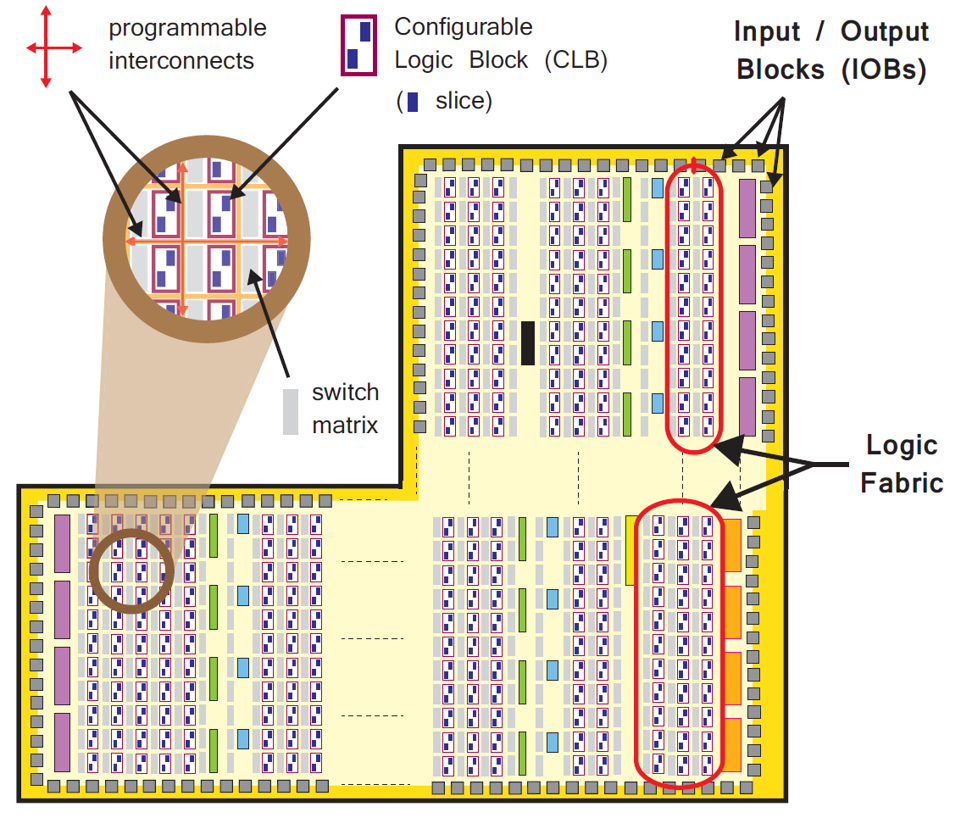
\includegraphics[width=0.5\textwidth]{images/Aufbau_PL.png}
    \end{figure}
    \ \\
\end{multicols}

\begin{multicols}{2}
    \subsection{Design Herausforderungen und Bedarf}
    \subsubsection{Herausforderungen}
    \begin{compactitem}
        \item Komplexität: Hohe Parallelität auf versch. Ebenen
        \item Heterogenität: Tools / Komponenten / Hersteller / Hardwarebeschreibung / Programmiersprache
        \item Time to market: Marktdruck
    \end{compactitem}
    \subsubsection{Bedarf}
    \begin{compactitem}
        \item Wiederverwendbarkeit: Systemfunktionalität kann nicht länger von Anfang an entwickelt werden $\rightarrow$ Komponenten und Subsysteme wiederverwenden $\rightarrow$ IP-basiertes Design
        \item Hierarchie: Weitere Hierarchiestufen sind erforderlich (sowohl Hard- wie auch Software) $\rightarrow$ IP-basiertes Design
        \item Parallel statt sequentiell: Hard- und Software sind parallel zu entwickeln
        \item Teams und Tools: Entwerfen von Systemen fordert grosse Teams und gute Werkzeuge, die die Komplexität verwalten können
    \end{compactitem}

    \ \\ \ \\
\end{multicols}

\begin{multicols}{2}
    \subsection{Traditioneller Design Flow}
     \begin{figure}[H]
     	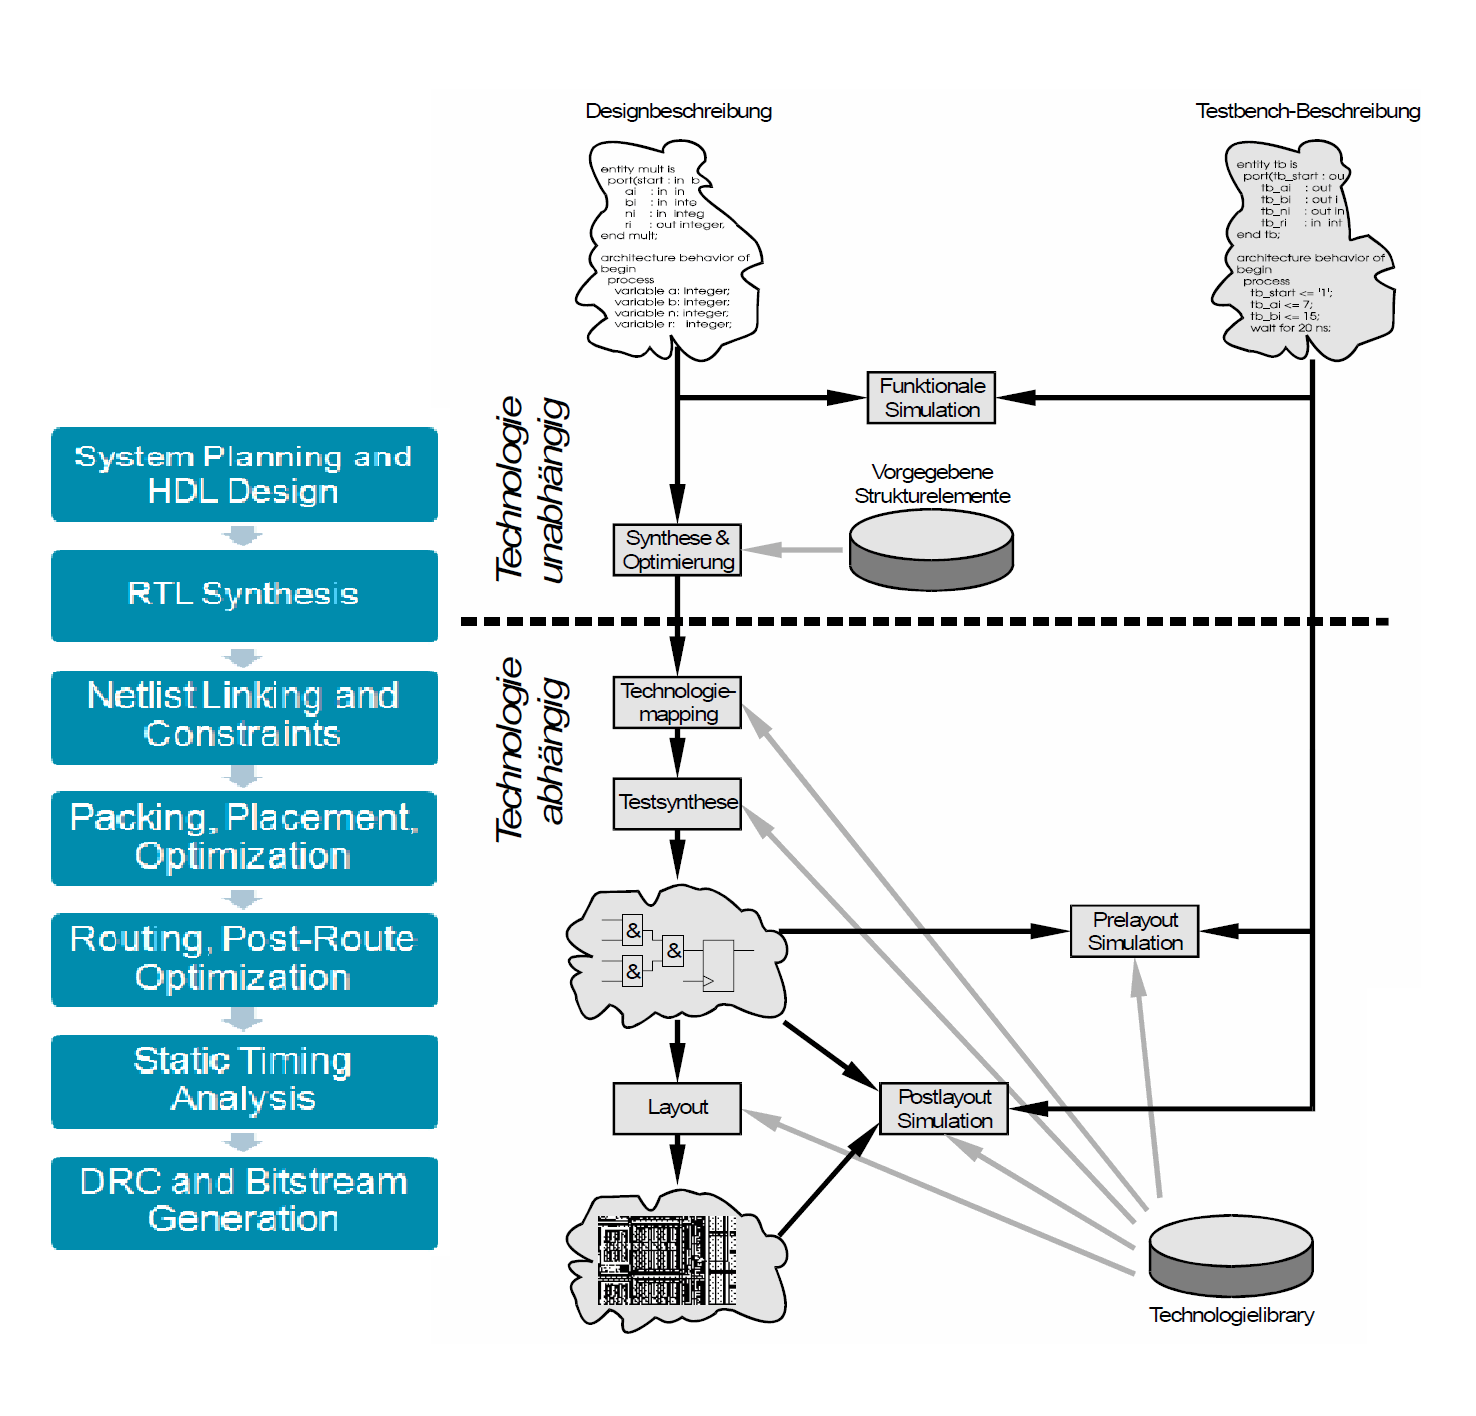
\includegraphics[width=0.53\textwidth]{images/Design_Flow_traditionell.png}
     \end{figure}
     \ \\ \ \\
    \subsection{System Level Design Flow}
    \begin{compactitem}
        \item Höhere Abstraktionsebene
        \item Partitionierung der SW und HW und Schnittstellendefinition
        \item SW/HW Co-Design
        \item System Integration $\rightarrow$ wird häufig unterschätzt
    \end{compactitem}
    \begin{figure}[H]
     	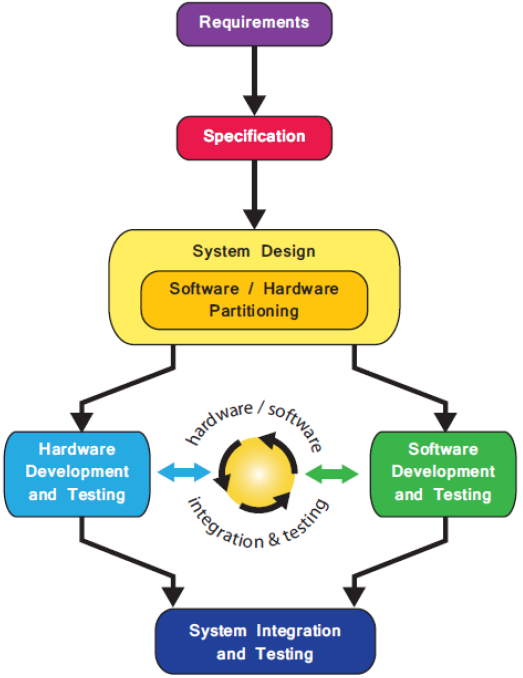
\includegraphics[width=0.35\textwidth]{images/Design_Flow_System_Level.png}
     \end{figure}
\end{multicols}
 \subsection{Design Tools}
 \subsubsection{Vivado IDE Solution}
 \paragraph{Haupteigenschaften}
 \begin{compactitem}
     \item Interaktives Design und Analyse: Timing Analysen, Konnektivität, Ressourcen Nutzung, Timinig Constraints Analysen, ..
     \item RTL Entwicklung und Analyse: Entwicklung von HDL, Hierarchische Erweiterung, Schemaerzeugung
     \item XSIM-Simulator-Integration
     \item Synthese und Umsetzung in einem Package
     \item I/O-Pin-Planung: Interaktive regelbasierte I/O Zuordnung
 \end{compactitem}
 \begin{multicols}{2}
     \paragraph{Design Database}
     Prozesse greifen auf die darunterliegende Datenbank des Designs zu. Jeder Prozess modifiziert eine vorhandene Netzliste oder erstellt eine neue. Während des ganzen Entwurfprozesses werden verschiedene Netzlisten (Elaborated, Synthesized, Implemented) verwendet.
     \subsubsection{Xilinx Software Development Kit (XSDK)}
    XSDK ist ein separates Tool von Vivado und kann eigenständig für SW-Teams installiert werden. Es ist eine voll ausgestattete Software-Design-Umgebung.
     \begin{figure}[H]
     	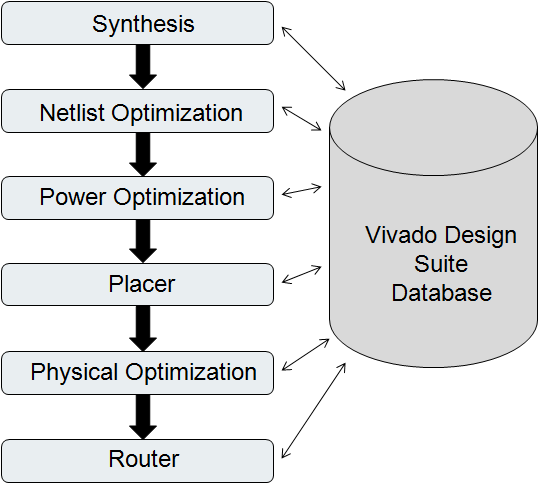
\includegraphics[width=0.25\textwidth]{images/Design_Database.png}
     \end{figure}
 \end{multicols}

\section{Constraints}
\subsection{``.xdc''-Dateien}$~$ \\
Physikalische Eigenschaften eines Designs können dem Synthese- und Implementierungstool mit Constraints mitgeteilt werden. Diese Constraints werden bei Vivado in ``.xdc''-Dateien definiert. Sind mehrere Dateien vorhanden, so werden diese sequentiell angewendet. Wird ein Constraint mehrfach gesetzt, so wird der zuletzt gesetzte Constraint verwendet. Für jede ``.xdc''-Datei kann desweiteren definiert werden, ob sie nur in der Synthese oder nur der Implementation angewendet werden soll (oder bei beidem).
\lstinputlisting[language=tcl,style=tcl]{code/tcl/xdc_property_used_in.xdc}

\subsubsection{Reihenfolge}
Es wird empfohlen die Constraints in der nachfolgenden Reihenfolge in den Dateien abzulegen, um Fehler zu minimieren.
\begin{multicols}{3}
    \begin{compactenum}
        \item Timing Assertions
        \begin{compactenum}
            \item Primary Clocks
            \item Virtual Clocks
            \item Generated Clocks
            \item Clock Groups
            \item Input und Output Delay
        \end{compactenum}
        \item Timing Exceptions
        \begin{compactenum}
            \item False Paths
            \item Max Delay / Min Delay
            \item Multicycle Paths
            \item Case Analysis
            \item Disable Timing
        \end{compactenum}
        \item Physical Constraints \\ \ \\ \ \\ \ \\
    \end{compactenum}
\end{multicols}

\subsection{Timing Analysis}$~$ \\
Um Constraints bestimmen zu können, muss als erstes eine Timing Analyse durchgeführt werden. Eine Timing Analyse soll sicherstellen, dass alle Timing Anforderungen aller Komponenten eingehalten werden. \\
\begin{minipage}{0.65\textwidth}
    \begin{figure}[H]
        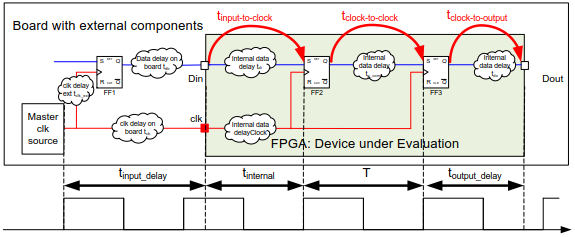
\includegraphics[width=\textwidth]{images/static_timing_analysis.png}
    \end{figure}
\end{minipage}
\hfill
\begin{minipage}{0.3\textwidth}
    Eine statische Timing Analyse muss die nachfolgenden Situationen abdecken:
    \begin{compactitem}
        \item Clock-to-Clock Pfad
        \item Input-to-Clock Pfad
        \item Clock-to-Output Pfad
    \end{compactitem}
    \ \\ \ \\ \ \\ \ \\ \ \\
\end{minipage}
\hspace*{+1cm}
\begin{multicols}{2}
    \subsubsection{Input Delay}
    Das Input Delay kann mit der nachfolgenden Formel bestimmt werden, weiterführende Informationen sind in Kapitel \ref{chapter:input_delay} zu finden. \\
    $t_{\text{input\_delay}}=t_{\text{clk\_ext}}+t_{\text{pcq\_FF1}}+t_{\text{db}}-t_{\text{cb}}$

    \subsubsection{Output Delay}
    Das Output Delay kann mit der nachfolgenden Formel bestimmt werden, weiterführende Informationen sind in Kapitel \ref{chapter:output_delay} zu finden. \\
    $t_{\text{output\_delay}}=t_{\text{pcq\_FF3}}+t_{\text{p\_comb}}+t_{\text{clk\_latency(FF3-master)}}$
\end{multicols}

\begin{multicols}{2}
    \subsubsection{Clock Skew}
    Der Skew ist die Timing Differenz zwischen zwei Signalen. Der Clock Skew ist die Differenz zwischen zwei Clock Signalen. Dieser Clock Skew sollte im Idealfall immer 0 sein. Da dies aber nicht realisierbar ist, implementieren die Synthesetools Clock Trees um den Clock Skew zu minimieren. Typischerweise ist der Clock Skew somit im Bereich von ps bis ns.
    \ \\ \ \\
    \begin{figure}[H]
        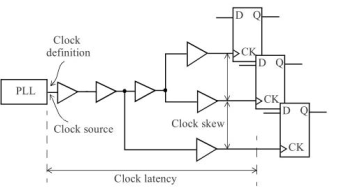
\includegraphics[width=0.35\textwidth]{images/clock_skew.png}
    \end{figure}
\end{multicols}

\subsubsection{Slack}
Der Slack bezeichnet die Differenz zwischen der benötigten Ankunftszeit eines Signales und der tatsächlichen Ankunftszeit. Solange der Slack einen positiven Wert aufweist, ist das Timing korrekt. Wird der Slack negativ, so können Timinganforderungen nicht mehr eingehalten werden.

\paragraph{Berechnung}$~$ \\
\begin{minipage}{0.3\textwidth}
    \begin{figure}[H]
        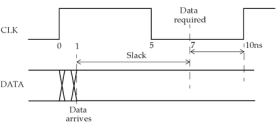
\includegraphics[width=1\textwidth]{images/slack.png}
    \end{figure}
\end{minipage}
\hfill
\begin{minipage}{0.65\textwidth}
    $Slack=RequiredTime-ArrivalTime$ wobei $RequiredTime=Tperiod-Tsetup(CaptureFlipFlop)$ \\
    Nach nebenstehendem Bild: $RequiredTime=10ns-3ns=7ns$ und $ArrivalTime=1ns$ ergibt $Slack=7ns-1ns=6ns$
\end{minipage}

\subsection{Clocks}$~$ \\
Clocks müssen definiert werden, damit die Timing Paths berechnet werden können. Ein Clock wird dabei so definiert, wie er am Startpunkt des Clock Trees aussieht (in der Regel der Eingangspin des Clocks). Es wird angegeben, wie gross die Periode des Clocks ist, sowie wo die Flanken sind. Alle Zeiten werden dabei in Nanosekunden angegeben.

\subsubsection{Primary Clocks}
Ein Primary Clock ist ein Clock, welcher in der Regel durch einen Eingangspin zugeführt wird. Ein solcher Clock muss immer einem Netzlistenobjekt zugewiesen werden. \\
Der nachfolgende Befehl definiert einen neuen Clock mit dem Namen \textit{devclk}, einer Periode von 10ns sowie einem Dutycycle von 25\%. Der Clock wird über den Port \textit{clkin} zugeführt.
\lstinputlisting[language=tcl,style=tcl]{code/tcl/primary_clock.xdc}

\subsubsection{Generated Clocks}
Generated Clock werden von speziellen Blöcken in einem FPGA generiert (z.B. MMCM). Sie können auch von Userlogik erzeugt werden. Diese Generated Clocks sind jedoch an einen anderen Clock gebunden und teilen diesen z.B. herunter, oder bewirken eine Phasenverschiebung.

\subsubsection{Virtual Clocks}
Ein Virtual Clock ist ein Clock welcher physikalisch nicht existiert und somit nicht an ein Netzlisten-Objekt gebunden ist. Sie werden benutzt um Input- und Output-Delays zu spezifizieren, wenn das externe Gerät mit einem anderen Clock läuft als der FPGA. \\
Der nachfolgende Befehl definiert einen neuen Virtual Clock mit dem Namen \textit{virtclk}, einer Periode von 10ns sowie einem Dutycycle von 25\%.
\lstinputlisting[language=tcl,style=tcl]{code/tcl/virtual_clock.xdc}

\subsubsection{Clock Latency}
\begin{minipage}{0.5\textwidth}
    \begin{figure}[H]
        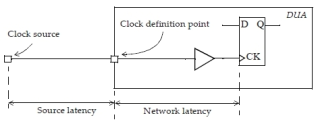
\includegraphics[width=1\textwidth]{images/clock_latency.png}
    \end{figure}
\end{minipage}
\hfill
\begin{minipage}{0.45\textwidth}
    Clocks erreichen verschiedene Punkte in einem Design mit unterschiedlichen Verzögerungen. Diese Verzögerungen können in zwei Arten unterschieden werden:
    \begin{compactitem}
        \item Network Latency
        \item Source Latency
    \end{compactitem} \ \\ \ \\
\end{minipage}

Mit den nachfolgenden Befehlen können die Latenzen definiert werden. Wird nichts spezifisch angegeben, so werden der  \textit{min}, \textit{max}, \textit{rise} und \textit{fall} Wert gesetzt.
\lstinputlisting[language=tcl,style=tcl]{code/tcl/clock_latency.xdc}

\subsubsection{Clock Jitter}
\begin{minipage}{0.3\textwidth}
    \begin{figure}[H]
        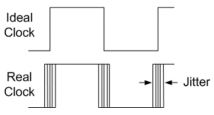
\includegraphics[width=1\textwidth]{images/clock_jitter.png}
    \end{figure}
\end{minipage}
\hfill
\begin{minipage}{0.65\textwidth}
    Aufgrund der physikalischen Eigenschaften ist kein Clock ideal. Kleinere Schwankungen in der Übertragung können auftreten. Diese Schwankungen werden Jitter genannt und in Nanosekunden gemessen. \ \\ \ \\ \ \\
\end{minipage}

\paragraph{Input Jitter}$~$ \\
Input Jitter definiert Jitter auf Primary Clocks. Mit dem nachfolgenden Befehl kann der Jitter definiert werden:
\lstinputlisting[language=tcl,style=tcl]{code/tcl/input_jitter.xdc}

\paragraph{System Jitter}$~$ \\
Der System Jitter spezifiert den Jitter für alle Clocks im System (auch für die Primary Clocks). Er wird benutzt um starkes Rauschen zu modellieren. Mit dem nachfolgenden Befehl kann der Jitter definiert werden:
\lstinputlisting[language=tcl,style=tcl]{code/tcl/system_jitter.xdc}

\begin{multicols}{2}
    \subsubsection{Zusätzliche Clock Unsicherheit}
    Sind weitere Unsicherheiten zwischen verschiedenen Clocks vorhanden, so kann mit dem nachfolgenden Befehl definiert werden, wie sich verschiedene Clocks zueinander verhalten.
    \lstinputlisting[language=tcl,style=tcl]{code/tcl/clock_uncertainty.xdc}
    \begin{figure}[H]
        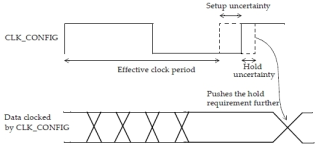
\includegraphics[width=0.5\textwidth]{images/clock_uncertainty.png}
    \end{figure}
\end{multicols}

\subsection{I/O Pin Constraints}
\lstinputlisting[language=tcl,style=tcl]{code/tcl/io_pin_constraints.xdc}

\subsection{I/O Delay}$~$ \\
Damit externe Timing-Anforderungen korrekt in die Synthese und Implementation einbezogen werden können, ist es notwendig diese anzugeben.

\subsubsection{Input Delay} \label{chapter:input_delay}
Input Delays geben an, mit welcher Verzögerung Daten an einem Eingangsport anliegen. Diese Verzögerung muss relativ zu einem Clock angegeben werden.

\paragraph{Tcl Befehl}$~$ \\
Mit dem Befehl \texttt{set\_input\_delay} kann das Input-Delay angegeben werden. Die folgenden Parameter werden dabei unterstützt:
\begin{compactitem}
    \item \texttt{-clock}: Gibt den Clock an, zu welchem die Verzögerung gilt.
    \item \texttt{-min}, \texttt{-max}: Definiert die min Zeit (hold/removal) oder die max Zeit (setup/recovery). Wird dieser Parameter nicht spezifisch angegeben, so wird die Input-Delay-Zeit für min und max verwendet.
    \item \texttt{-clock\_fall}: Gibt an, dass der Input-Delay relativ zur fallenden Clockflanke gilt.
    \item \texttt{-rise}, \texttt{-fall}: Gibt an, für welche Flanke des Eingangssignales die Angaben gelten.
    \item \texttt{-add\_delay}: Diese Option wird benutzt, wenn ein zweites Delay angegeben werden muss (z.B. bei DDR).
\end{compactitem}

\paragraph{Beispiel}$~$ \\
\begin{figure}[H]
    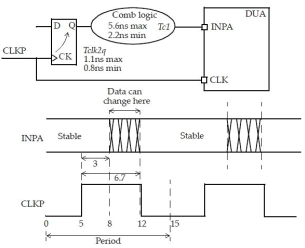
\includegraphics[width=0.5\textwidth]{images/input_delay.png}
\end{figure}
\lstinputlisting[language=tcl,style=tcl]{code/tcl/input_delay.xdc}

\subsubsection{Output Delay} \label{chapter:output_delay}
Output Delays geben an, in welchem Zeitbereich die Daten am Ausgangsport stabil sein müssen. Dieser Zeitbereich wird wiederum relativ zu einem Clock angegeben.

\paragraph{Tcl Befehl}$~$ \\
Mit dem Befehl \texttt{set\_output\_delay} kann das Output-Delay angegeben werden. Die folgenden Parameter werden dabei unterstützt:
\begin{compactitem}
    \item \texttt{-clock}: Gibt den Clock an, zu welchem die Zeit gilt.
    \item \texttt{-min}, \texttt{-max}: Definiert die min Zeit (hold/removal) oder die max Zeit (setup/recovery). Wird dieser Parameter nicht spezifisch angegeben, so wird die Input-Delay-Zeit für min und max verwendet.
    \item \texttt{-clock\_fall}: Gibt an, dass der Output-Delay relativ zur fallenden Clockflanke gilt.
    \item \texttt{-rise}, \texttt{-fall}: Gibt an, für welche Flanke des Ausgangssignales die Angaben gelten.
    \item \texttt{-add\_delay}: Diese Option wird benutzt, wenn ein zweites Delay angegeben werden muss (z.B. bei DDR).
\end{compactitem}

\paragraph{Beispiel}$~$ \\
\begin{figure}[H]
    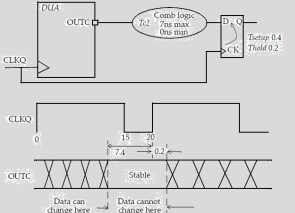
\includegraphics[width=0.5\textwidth]{images/output_delay.png}
\end{figure}
\lstinputlisting[language=tcl,style=tcl]{code/tcl/output_delay.xdc}

\section{System Level VHDL}
\subsection{Wiederverwendbarkeit}
Bereits auf der untersten Abstraktionsebene soll wiederverwendbarer Code geschrieben werden. Um einen Code wiederverwenden zu können, muss dieser gut lesbar sein. Nachfolgend ein paar Hilfsmittel um den Code gut lesbar zu gestalten.
\subsubsection{Kommentare}
Zeilenkommentare $\rightarrow$ beginnen mit -{}-\\
Blockkommentare $\rightarrow$ beginnen mit /* und enden mit */
\subsubsection{Namenskonventionen}
In VHDL sind keine Namenskonventionen definiert. Es wird jedoch empfohlen folgende Mindestregeln einzuhalten: 
\begin{compactitem}
    \item Aussagekräftige Namen für Entitys, Architekturen, Funktionen und Prozesse verwenden
    \item Namen sollten lowercase sein und zum trennen von Wörtern sollte man Underscores verwenden
    \item Entitys sollten eindeutige Namen haben. Architekturen benötigen keine eindeutigen Namen. Ihr Name beschreibt eher die Natur der Architektur wie RTL, Struktur usw
    \item Signalnamen sollten lowercase sein und zum trennen von Wörtern sollte man Underscores verwenden 
    \item Low-Aktive Signale sollten deutlich als solche im Signalnamen markiert werden (\textit{XXXX\_l} oder \textit{XXXX\_n})
\end{compactitem}
Spezielle Namenskonventionen ermöglichen es dem Vivado IP-Packager, automatisch AXI-Schnittstellensignale abzuleiten: 
\begin{compactitem}
    \item Reset: \_reset, \_rst, \_resetn (low-aktiv), \_areset 
    \item Clock: \_clk, \_clkin, \_clk\_p (Diff. Clock), \_clk\_n (Diff. Clock)
    \item AXI Interface: \_tdata (Bsp: s0\_axis\_tdata), \_tvalid, \_tready
\end{compactitem}
\subsubsection{Einsatz von Konstanten}
Wenn möglich nie Parameter gebrauchen! Konstanten sind im Bezug auf die Änderbarkeit unverzichtbar. Konstanten in VHDL-Packages können in mehreren Designeinheiten verwendet werden. Konstanten, die in Designentitäten (Deklarationsteil der Architektur) deklariert sind, können in der gesamten Architektur einschliesslich der Prozesse innerhalb dieser Architektur gesehen werden. Der Scope einer Konstante, welche in einem Prozess deklarierten wurde, ist auf diesen Prozess beschränkt.
\lstinputlisting[language=VHDL]{code/constants.vhd}
\subsubsection{Einsatz von Aliases}
\lstinputlisting[language=VHDL]{code/aliases.vhd}
\subsubsection{Einsatz von Generics}
Generics werden zu Beginn der Entity deklariert.
\lstinputlisting[language=VHDL]{code/generics.vhd}

\subsection{Funktionen}
Funktionen sind Subprogramme mit einer Argumentenliste von nur Eingängen. Sie geben einen einzigen Wert eines spezifizierten Types zurück. Funktionen können entweder im Deklarationsteil einer Architektur oder in einem Package (flexibler) definiert werden. 
\lstinputlisting[language=VHDL]{code/functions.vhd}
\textbf{Wichtig:}
\begin{compactitem}
    \item Im Funktionsblock dürfen keine wait-Anweisungen oder Signalzuweisungen enthalten sein! 
    \item := wird verwendet, wenn ein Wert einer \textbf{Variablen} zugewiesen wird. Wird sofort in einem Prozess zugeordnet.
    \item \textless= wird verwendet, wenn ein Signal einem Signal zugewiesen wird. Wird am Ende eines Prozesses zugewiesen.
\end{compactitem}
\textbf{Unterschied pure und impure Funktionen:} Bei Funktionen, welche pure sind, bekommt man bei jedem Aufruf für jeden Input den gleichen Output (z.B. sin(x)). Bei impuren Funktionen erhält man bei gleichem Input unterschiedliche Outputs. Impure Funktionen haben Seiteneffekte, wie z.B. das Updaten von Objekten ausserhalb ihres Scopes, was bei puren Funktionen nicht erlaubt ist.
\lstinputlisting[language=VHDL]{code/functions_impure.vhd}

\subsection{Prozeduren}
Prozeduren sind sehr ähnlich wie Funktionen. Der Hauptunterschied ist, dass bei Prozeduren mehrere Ein- und Ausgangsvariablen definiert werden können. 
\lstinputlisting[language=VHDL]{code/procedures.vhd}
\textbf{Wichtig: }
\begin{compactitem}
    \item Prozeduren können In-, Out- oder Inout-Parameter besitzen. Diese können ein Signal, eine Variable oder eine Konstante sein. Die Voreinstellung für in-Parameter ist konstant, für out und inout variabel.
\end{compactitem}

\subsection{Packages}
Konstanten, Typen, Komponenten, Funktionen und Prozeduren, die an verschiedenen Stellen in einem oder mehreren Projekten verwendet werden, können in Packages gruppiert werden.
\lstinputlisting[language=VHDL]{code/packages.vhd}
Packages werden in Bibliotheken kompiliert abgelegt (Standard = work library). Sie können im VHDL-Modul mit der use-Anweisung verwendet werden:
\lstinputlisting[language=VHDL]{code/packages_use.vhd}

\subsection{IP Blöcke}
\subsubsection{Konfiguration von IP Blöcken}
\begin{compactitem}
    \item IP Blöcke sind meistens konfigurierbare Module. Jede Instanz eines solchen IP Blocks kann individuell konfiguriert werden.
    \item Konfiguration von Hard IP Blöcke: Beschränkt auf das Ein- und Ausschalten bestimmter Funktionen, da Hardware nicht modifiziert werden kann.
    \item Konfiguration von Soft und Firm IP Blöcke: Flexibler, da diese Blöcke erst nach der Konfiguration synthetisiert werden. Häufig kann Funktionalität, Implementierungsstrategie, Schnittstellentyp und Dimensionen eingestellt werden. Konfigurationsparameter werden als generische Parameter an das Modul zur Synthese übergeben.  
\end{compactitem}
\subsubsection{IP Packager}
\begin{compactitem}
    \item IP Blöcke bestehen aus vielen Teilen: 
    \begin{compactitem}
        \item Quelldateien (RTL, C-Code, Netzlistendateien etc.) 
        \item Dokumentation
        \item Simulationsmodelle
        \item Testbenches
        \item Beispiele
    \end{compactitem} 
    \item Vivado IP Packager stellt aus obigen Teilen ein Komplettpaket zusammen und legt es in ein zentrales Repositiory (IP Katalog).
    \item IP-XACT: Standard (in XML) für die Verpackung und Dokumentation, welcher von einer Gruppe aus IP-Anbietern unter dem Namen SPIRIT Consortium definiert wurde. Beschreibt nur Schnittstelle und Organisation des Blocks und bietet damit eine Zugangstür für die verschiedenen Werkzeuge, um ihre Informationen zu finden.
    \item component.xml: Enthält Metadaten, Ports, Schnittstellen, Konfigurationsparameter, Dateien und Dokumentation beschrieben. Ersetzt nicht HDL oder Software (enthält nur High-Level-Informationen).  
\end{compactitem}
\subsubsection{Einbinden von IP Blöcken in eigenes Design}
\begin{compactenum}
    \item IP Repository (normalerweise in Projekt oder auf Firmenlaufwerk) dem Projekt bekannt machen.
    \item IP Block aus Katalog auswählen (add IP).
    \item Anpassungen und Generierung spezifischer Ausgabeprodukte (output products): Anpassung erfolgt im IP Integrator. Die Parameter müssen an den RTL-Code des IP Blockes übergeben werden und der Code muss in  das Design aufgenommen werden. Bei Generierung der Ausgabeprodukte erzeugt der IP Integrator die kundenspezifischen Designinformationen.
    \item IP verwenden: Der Baustein kann nun verwendet werden, indem er mit dem IP-Integrator im Blockdesign platziert oder in einem herkömmlichen RTL-Design instanziiert wird. 
\end{compactenum}
IP Blöcke können verschieden eingebunden werden:
\begin{compactitem}
        \item Via IP Integrator: Vivado führt die folgenden Schritte aus: Instanziierung (Block einfügen in Design), Erzeugung von System-Wrapper (strukturelle VHDL-Top-Level-Beschreibung) und Generierung der Ausgabeprodukte.
        \item Via Instanzierungs-Template im RTL Flow: Für VHDL und Verilog werden Instanzierungs-Templates zur Verfügung gestellt. Der IP Block muss in der Design-Datei, welche eine Position höher in der Design-Hierarchie ist, instanziiert werden.   
\end{compactitem}
\lstinputlisting[language=VHDL]{code/component.vhd}
\subsubsection{IP Life Cycle}
\begin{compactitem}
        \item Vorproduktion (pre-production): IP Core, der öffentlich verwendbar ist, aber noch keine Qualifikationen für den Einsatz in der Produktion aufweist.
        \item Produktion (production): IP Core, der für die allgemeine öffentliche Freigabe zur Verfügung gestellt wird und verifiziert wurde. 
        \item Eingestellt (discontinued): Ankündigung von XILINX, dass IP Core bald entfernt wird.
        \item Ersetzt (superseded): IP Core wurde durch eine neuere Version ersetzt.
        \item Entfernt (removed): IP Core wird nicht mehr länger vertrieben.
\end{compactitem}

\section{Fixed Point Arithmetic}
\subsection{Einleitung}$~$ \\
\begin{tabular}{| l | l | l |}
\hline
& Unsigned integer & Signed integer\\
\hline
Formel & $z=\sum_{k=0}^{n-1}a_k \cdot 2^k$ & $z=-(2^{n-1}) \cdot a_{n-1} + \sum_{k=0}^{n-2}2^k \cdot a_k$\\
\hline
Bereich & $0 \ldots 2^n-2^0$ & $-2^{n-1} \ldots 2^{n-1}-2^0$\\
\hline
\end{tabular}

\subsection{Qn.m Format}$~$ \\
n: Anzahl integer bits (inkl. eines allfälligen Vorzeichenbits); m: Anzahl der Nachkommastellen\\
Es gibt zwei Möglichkeiten, eine Fix-point Zahl in VHDL zu implementieren:
\begin{compactitem}
  \item Nur mit dem 'numeric\_std'-Package und dabie unsigned und signed Typen zu verwenden. Der Programmierer muss praktisch alles selbst machen (z.B. Dezimalpunkt tracken)
  \item Mithilfe des 'fixed\_pkg-Packages' (basiert auf 'numeric\_std') $\rightarrow$ einfacherer, übersichtlicherer Code; fast alle Operatoren sind für integer und reelle Typen überladen; Overflows sind nicht möglich $\rightarrow$ führt immer zu sicherer Implementation, aber nicht immer zur optimalen Lösung in Bezug auf die Vektorbreite
\end{compactitem}
Sizing-Regeln für 'fixed\_pkg':\\
\begin{tabular}{| l | l |}
\hline
Operation & Result Range\\
\hline
$A+B$ & Max(A'left,B'left)+1 downto Min(A'right,B'right)\\
\hline
$A-B$ & Max(A'left,B'left)+1 downto Min(A'right,B'right)\\
\hline
$A \cdot B$ & A'left+B'left+1 downto A'right+B'right\\
\hline
$A \text{ rem } B$ & Min(A'left,B'left)+1 downto Min(A'right,B'right)\\
\hline
$\text{Signed } /$ & A'left-B'right+1 downto A'right-B'left\\
\hline
$\text{Signed A mod B}$ & Min(A'left,B'left) downto Min(A'right,B'right)\\
\hline
$\text{Signed Reciprocal(A)}$ & -A'right downto -A'left-1\\
\hline
$\text{Abs(A)}$ & A'left+1 downto A'right\\
\hline
$-A$ & A'left+1 downto A'right\\
\hline
$\text{Unsigned} /$ & A'left-B'right downto A'right-B'left-1\\
\hline
$\text{Unsigned A mod B}$ & B'left downto Min(A'right,B'right)\\
\hline
$\text{Unsigned Reciprocal(A)}$ & -A'right+1 downto -A'left\\
\hline
\end{tabular}

\subsubsection{ufixed/sfixed}
Das Package definiert zwei neue Datentypen: ufixed und sfixed. Für negative zahlen wird das 2er-Komplement verwendet. Die Position des Dezimalpunkts ist zwischen Index ''0'' und ''-1''.
\lstinputlisting[language=VHDL,style=VHDL]{code/ufixed_sfixed.vhd}

\subsubsection{Limitierte Unterstützung}
Das Package ist Teil von VHDL 2008, weshalb es von gewissen Tools noch nicht vollständig unterstützt wird. XILINX bietet eine modifizierte Version von 'fixed\_pkg' an.
\lstinputlisting[language=VHDL,style=VHDL]{code/fixed_pkg.vhd}

\subsubsection{Unsigned/Signed}
\begin{tabular}{| l | l | l |}
\hline
&  uQn.m & uQn.m\\
\hline
Formel & $z=\sum_{k=-m}^{n-1}a_k \cdot 2^k$ & $z=-(2^{n-1}) \cdot a_{n-1} + \sum_{k=-}^{n-2}a_k \cdot 2^k$\\
\hline
Bereich & $0 \ldots 2^n-2^{-m}$ & $-2^{n-1} \ldots 2^{n-1}-2^{-m}$\\
\hline
\end{tabular}\\
\textbf{Bsp.: uQ2.6}
\lstinputlisting[language=VHDL,style=VHDL]{code/uQ2_6.vhd}
\textbf{Bsp.: sQ2.6}
\lstinputlisting[language=VHDL,style=VHDL]{code/sQ2_6.vhd}

\subsection{Arithmetic Functions}
\subsubsection{Addition/Subtraction}
\paragraph{Unsigned and Unsigned}$~$ \\
\begin{minipage}{0.3\linewidth}
Praktisch identisch mit Add./Sub. mit normalen Integer-Zahlen, einzig muss nun der Programmierer den Dezimalpunkt tracken.
\end{minipage}
\begin{minipage}{0.7\linewidth}
\begin{tabular}{l l l l l l l l l | l}
& \textbf{0} & 1 & 0 & 1 & 1 & 0 & 1 & \textbf{0} & = 101.101 in uQ3.3 = 5.625\\
+ & & & & 1 & 0 & 0 & 1 & 1 & = 1.0011 in uQ1.4 = 1.1875\\
\hline
& \textbf{0} & 1 & 1 & 0 & 1 & 1 & 0 & 1 & = 0110.1101 in uQ4.4 = 6.8125\\
\end{tabular}
\end{minipage}
\lstinputlisting[language=VHDL,style=VHDL]{code/addition_subtraktion.vhd}

\paragraph{Signed and Signed}$~$ \\
\begin{minipage}{0.3\linewidth}
Auch fast identisch, Zahl mit weniger Vorkommabits muss sign-extended werden
\end{minipage}
\begin{minipage}{0.7\linewidth}
  \begin{tabular}{l l l l l l l l l | l}
  & \textbf{1} & 1 & 0 & 1 & 1 & 0 & 1 & \textbf{0} & = 101.101 in sQ3.3 = -2.375\\
  + & \textbf{1} & \textbf{1} & \textbf{1} & 1 & 0 & 0 & 1 & 1 & = 1.0011 in sQ1.4 = -0.8125\\
  \hline
  & \textbf{1} & 1 & 0 & 0 & 1 & 1 & 0 & 1 & = 1100.1101 in sQ4.4 = -3.1875\\
  \end{tabular}
\end{minipage}
\lstinputlisting[language=VHDL,style=VHDL]{code/addition_subtraktion_signed.vhd}

\subsubsection{Multiplication}
\paragraph{Unsigned by Unsigned}$~$ \\
Einfachster Fall, partielle Produkte werden ohne sign-extension addiert\\
\begin{minipage}{0.7\linewidth}
  \begin{tabular}{ l l l l l l l l | l}
  & & & & 1 & 1 & 0 & 1 & = 11.01 in uQ2.2 = 3.25 (multiplicand)\\
   & & & 1 & 0 & 1 & 1 & = 10.11 in uQ2.2 = 2.75 (multiplier)\\
  \hline
  & & & & 1 & 1 & 0 & 1 & \\
  & & & 1 & 1 & 0 & 1 & & \\
  & & 0 & 0 & 0 & 0 & & & \\
  & 1 & 1 & 0 & 1 & & & & \\
  \hline
  1 & 0 & 0 & 0 & 1 & 1 & 1 & 1 & = 1000.1111 in uQ4.4 = 8.9375
  \end{tabular}
\end{minipage}
\lstinputlisting[language=VHDL,style=VHDL]{code/multiplikation_unsigned.vhd}

\paragraph{Signed by Unsigned}$~$ \\
Hier braucht jedes partielle Produkt sign-extension. In VHDL ist $\text{signed} \cdot \text{unsigned}$ nicht erlaubt. Der vorzeichenlose Wert muss zuerst in eine vorzeichenbehaftete Zahl gewandelt werden.\\
\begin{minipage}{0.7\linewidth}
  \begin{tabular}{ l l l l l l l l | l}
  & & & & 1 & 1 & 0 & 1 & = 11.01 in sQ2.2 = -0.75 (multiplicand)\\
  & & & & 0 & 1 & 0 & 1 & = 01.01 in sQ2.2 = 1.25 (multiplier)\\
  \hline
  \textbf{1} & \textbf{1} & \textbf{1} & \textbf{1} & 1 & 1 & 0 & 1 & \\
  \textbf{0} & \textbf{0} & \textbf{0} & 0 & 0 & 0 & 0 & & \\
  \textbf{1} & \textbf{1} & 1 & 1 & 0 & 1 & & & \\
  \textbf{0} & 0 & 0 & 0 & 0 & & & & \\
  \hline
  1 & 1 & 1 & 1 & 0 & 0 & 0 & 1 & = 1111.0001 in sQ4.4 = -0.9375
  \end{tabular}
\end{minipage}

\paragraph{Signed by Signed}$~$ \\
Zwei Möglichkeiten:
\begin{compactitem}
  \item Sign-extension aller partiellen Produkte. Wenn der 'multiplier' negativ ist, muss das letzte partielle Produkt mit dem 2er-Komplement transformiert werden.
  \item Beide Zahlen werden mit dem 2er-Komplement transformiert. Das partielle Produkt wird sign-extended, wenn der neue 'multiplicand' negativ ist.
\end{compactitem}
Das MSB des Produkts ist redundant. Wird das Produkt nach links geschoben, kann das redundante Bit entfernt und ein zusätzliches fractional bit hinzugefügt werden (neues Format: Q(n1+n2-1).(m1+m2+1)).\\
\begin{minipage}{0.7\linewidth}
  \begin{tabular}{ l l l l l l l l | l}
  & & & & 0 & 1 & 0 & 1 & = 01.01 in sQ2.2 = 1.25 (multiplicand)\\
  & & & & 1 & 0 & 1 & 1 & = 10.11 in sQ2.2 = -1.25 (multiplier)\\
  \hline
  \textbf{0} & \textbf{0} & \textbf{0} & \textbf{0} & 0 & 1 & 0 & 1 & \\
  \textbf{0} & \textbf{0} & \textbf{0} & 0 & 1 & 0 & 1 & & \\
  \textbf{0} & \textbf{0} & 0 & 0 & 0 & 0 & & & \\
  \textbf{1} & 1 & 0 & 1 & 1 & & & & 2's complement of multiplicand 0101\\
  \hline
  1 & 1 & 1 & 0 & 0 & 1 & 1 & 1 & 110.01110 in sQ3.5 = -1.5625\\
  & & & & & & & & (one of the sign bits is removed)\\
  \end{tabular}
\end{minipage}\\
\begin{minipage}{0.7\linewidth}
  \begin{tabular}{ l l l l l l l l | l}
  & & & & 1 & 0 & 1 & 1 & = 2's complement of multiplicand 0101\\
  & & & & 0 & 1 & 0 & 1 & = 2's complement of multiplier 1011\\
  \hline
  \textbf{1} & \textbf{1} & \textbf{1} & \textbf{1} & 1 & 0 & 1 & 1 & multiplicand is negative $\rightarrow$ extended sign-bits\\
  \textbf{0} & \textbf{0} & \textbf{0} & 0 & 0 & 0 & 0 & & \\
  \textbf{1} & \textbf{1} & 1 & 0 & 1 & 1 & & & \\
  \textbf{0} & 0 & 0 & 0 & 0 & & & & \\
  \hline
  1 & 1 & 1 & 0 & 0 & 1 & 1 & 1 & 110.01110 in sQ3.5 = -1.5625
  \end{tabular}
\end{minipage}\\.
\lstinputlisting[language=VHDL,style=VHDL]{code/multiplikation_signed.vhd}
\textbf{Corner case:} Wenn die zwei kleinst möglichen Zahlen multipliziert werden (bei sQ2.2: 1000*1000). Dies führt zu einem Overflow und zu einem falschen Ergebnis (-4 anstatt +4). $\rightarrow$ \textbf{Lösung:} Das zweite Vorzeichenbit als Schutz stehen lassen. Dies ist so auch im 'fixed\_pkg'-Package umgesetzt

\subsubsection{Division}
Divisionen mit Mehrfachen von 2 ($2^n$) sind einfache Schiebeoperationen. Für andere Werte ist es komplizierter. 'fixed\_pkg' bietet eine elegante Lösung an:
\lstinputlisting[language=VHDL,style=VHDL]{code/division.vhd}

\subsection{Overflow and Saturation}$~$ \\
Bei Verwendung des 'fixed\_pkg'-Packages werden Overflow und Saturation automatisch gelöst. Ansonsten gibt es zwei Lösungen mit einem Over-/Underflow umzugehen: Das Resultat sättigen (Maximum oder Minimum) oder das Resultat erhält ein zusätzliched integer bit.\\
Erkennung bei vorzeichenbehafteten Zahlen:
\begin{compactitem}
  \item Overflow, wenn Summe von zwei positiven Zahlen ein negatives Resultat liefert.
  \item Underflow, wenn Summe von zwei negativen Zahlen ein positives Resultat liefert.
  \item Die Summe einer positiven und negativen Zahl ergibt nie einen Underflow.
\end{compactitem}
Erkennung bei vorzeichenlosen Zahlen:
\begin{compactitem}
  \item Overflow, wenn Summe einer Addition kleiner als der erste Summand ist.
  \item Underflow, wenn Differenz einer Subtraktion grösser als der Subtrahend ist.
\end{compactitem}
\textbf{fixed\_pkg:} Der einzige Fall, dass ein Underflow entstehen kann, ist wenn das Resultat resized wird in eine kleiner Grösse. Die resize-Funktion von 'numeric\_std' wird überladen:
\lstinputlisting[language=VHDL,style=VHDL]{code/resize_fixed_pkg.vhd}
Mit der nun vorhandenen resize-Funktion ist es möglich, das Overflow-Handling, 'truncation' oder 'rounding' in einem Schritt durchzuführen. Der Default 'overflow\_style' ist 'fixed\_saturate', kann aber auch auf 'fixed\_wrap' zu setzen um einen Overflow zu ermöglichen. Der Default 'round\_style' ist 'fixed\_round' um das Resultat zu runden, kann aber auch auf 'fixed\_truncate' gesetzt werden.

\subsection{Scaling}$~$ \\
Das Resultat einer Multiplikation hat die Breite des 'multiplicand' plus 'multiplier', mehrere aufeinanderfolgende Multiplikationen führen somit zu Bit Growth.

\subsubsection{Truncation}$~$ \\
Eine Möglichkeit: Bits mit tiefer Präzision weglassen. Die normale 'truncation' ist eine floor-Funktion. In VHDL kann das mit 'shift\_right' und 'resize' umgesetzt werden:
\lstinputlisting[language=VHDL,style=VHDL]{code/truncation.vhd}

\section{Speicher - Custom IP Blocks}
\subsection{Typen von Speicher in FPGA}
In einem FPGA sind normalerweise zwei Arten von Speicher vorhanden:
\begin{compactitem}
    \item \textbf{Distributed Memory}: Distributed Memory besteht aus vielen LUT Tabellen. Der Vorteil dieser Variante ist, dass jede beliebige Grösse von Speicher realisiert werden kann. Desweitern kann dieser Speicher an jedem Ort in einem FPGA erstellt werden. Ideal für kleine Speichergrössen.
    \item \textbf{Block Memory}: Block Memory sind fest implementierte Speicherzellen (Hard IP Block). Diese bestehen aus SRAM Zellen (zwei kreuzgekoppelte Inverter) und sind über das ganze FPGA hinweg verteilt. Oftmals haben sie auch gerade eine Fehlerkorrektur implementiert (bei Xilinx: Hamming Error Correction Code). Ideal für grössere Speichergrössen. Die Speichergrösse bei den Xilinx Series 7 Block Rams beträgt 32kb (36kb physikalisch vorhanden).
\end{compactitem}

\subsubsection{ROM}
ROM wird benutzt um konstante Daten zu speichern. In einem FPGA wird die Implementierung von ROM mithilfe von RAM gemacht.

\subsubsection{Interface Arten}
Beide Speicherarten können mit zwei verschiedenen Schnittstellen implementiert werden.

\begin{minipage}{0.3\textwidth}
    \begin{figure}[H]
        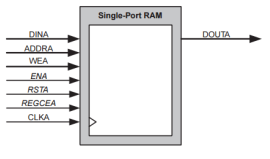
\includegraphics[width=1\textwidth]{images/singleportram.png}
    \end{figure}
\end{minipage}
\hfill
\begin{minipage}{0.65\textwidth}
    \paragraph{Single-Port RAM}
    Single-Port RAM hat einen Daten- und einen Adressbus. Darüber sind sequentielle Lese- und Schreibzugriffe möglich. Wird Distributed Memory verwendet, so ist es auch zusätzlich noch möglich asynchrone Lesezugriffe durchzuführen. \ \\ \ \\ \ \\
\end{minipage}

\begin{minipage}{0.3\textwidth}
    \begin{figure}[H]
        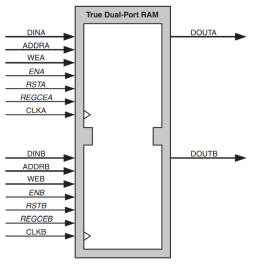
\includegraphics[width=1\textwidth]{images/dualportram.png}
    \end{figure}
\end{minipage}
\hfill
\begin{minipage}{0.65\textwidth}
    \paragraph{Dual-Port RAM}
    Dual-Port RAM erlaubt zwei gleichzeitige Lese- und/oder Schreibzugriffe. Wird über beide Schnittstellen auf die gleiche Speicherzelle zugegriffen, so gibt es eine Arbitrierschaltung, welche diese Situation korrekt abwickelt. \ \\ \ \\ \ \\ \ \\ \ \\ \ \\ \ \\ \ \\ \ \\ \ \\
\end{minipage}


\subsection{Beschreibung von Speicher in VHDL}
Es existieren vier Richtlinien für das Beschreiben von ROM und RAM in VHDL. Wird Speicher anhand dieser Richtlinien beschrieben, so sollte der Synthesizer den Speicher korrekt implementieren.
\begin{compactenum}
    \item Die Datengrösse und die Adressengrösse sollen mit generischen Parametern definiert werden.
    \item Der Addressenbereich soll mit einer Konstante definiert werden.
    \item RAM soll mit einem zweidimensionalen Array beschrieben werden.
    \item Der Schreibzugriff muss in einem Prozess beschrieben werden.
\end{compactenum}

\subsubsection{Block RAM - Single-Port}
\lstinputlisting[language=VHDL]{code/blockram_single.vhd}

\subsubsection{Distributed RAM - Single-Port}
\lstinputlisting[language=VHDL]{code/distributedram_single.vhd}

\subsubsection{Block RAM - Dual-Port}
\lstinputlisting[language=VHDL]{code/blockram_dual.vhd}

\subsubsection{ROM}
Da ROM gleich wie RAM implementiert wird, muss nur das RAM Signal als Konstante definiert werden.
\lstinputlisting[language=VHDL]{code/rom.vhd}

\subsubsection{Synthese-Attribute}
Mit dem Attribut \texttt{ram\_style} kann Vivado mitgeteilt werden, ob das RAM als Distributed RAM (\texttt{"distributed"}) oder als Block RAM (\texttt{"block"}) implementiert werden soll.
\lstinputlisting[language=VHDL]{code/ram_attribute.vhd}

\subsubsection{Initialisierung}
Eine einfache Art um Speicher zu initialisieren, kann mit Hilfe einer Funktion und einer Datei erreicht werden.
\lstinputlisting[language=VHDL]{code/rom_init.vhd}

Der Speicher kann aber auch direkt im Code initialisiert werden (eher aufwändig und unübersichtlich):
\lstinputlisting[language=VHDL]{code/ram_init2.vhd}

\subsection{Memory IP Generators}
Vivado stellt verschiedene IP Generatoren zur Verfügung, über welche direkt Speicher instanziiert werden kann. Diese Generatoren stellen eine einfache Möglichkeit dar, um Speicher nach den eigenen Wünschen zu konfigurieren. Ebenfalls stellen sie präzise Simulationsmodelle zur Verfügung.

\subsection{Intellectual Property IP}
\begin{multicols}{2}
\subsection{Definition IP Core}
Als IP Core (Intellectual Property Core) wird ein vielfach einsetzbarer, vorgefertigter Funktionsblock eines Chipdesigns bezeichnet. Dieser enthält das geistige Eigentum (intellectual property) des Entwicklers oder Herstellers und wird in der Regel lizenziert bzw. hinzugekauft, um es in ein eigenes Design zu integrieren.

\vfill\null
\columnbreak

\subsection{IP Core Typen}
\begin{compactitem}
    \item Hard IP Core: Blackbox in optimierter Layoutform. Sind als fertige Schaltung herstellerseitig unveränderbar in den Chip des FPGAs integriert
    \item Firm IP Core: Synthetisierte Netzliste, die simuliert und wenn nötig geändert werden kann
    \item Soft IP Core: RTL Design. Benutzer muss synthetisieren und layouten
\end{compactitem}
\end{multicols}

\begin{multicols}{2}
\subsection{Bezug von IP Core}
\begin{compactitem}
    \item Ältere bereits vorhandene in-house IP
    \item Neu entwickelte in-house IP
    \item Drittanbieter IP
\end{compactitem}

\vfill\null
\columnbreak

\subsection{Lizenzmodelle}
\begin{compactitem}
    \item Free und Open Source
    \item Kommerzielle Lieferanten (XILINX, CADENCE, ..)
    \item Aggregator (sammelt und kategorisiert IP Cores und verkauft sie weiter)
\end{compactitem}
\end{multicols}

\subsubsection{Konfiguration von IP Blöcken}
\begin{compactitem}
    \item IP Blöcke sind meistens konfigurierbare Module. Jede Instanz eines solchen IP Blocks kann individuell konfiguriert werden.
    \item Konfiguration von Hard IP Blöcken: Beschränkt auf das Ein- und Ausschalten bestimmter Funktionen, da Hardware nicht modifiziert werden kann.
    \item Konfiguration von Soft und Firm IP Blöcken: Flexibler, da diese Blöcke erst nach der Konfiguration synthetisiert werden. Häufig können Funktionalität, Implementierungsstrategie, Schnittstellentyp und Dimensionen eingestellt werden. Konfigurationsparameter werden als generische Parameter an das Modul zur Synthese übergeben.
\end{compactitem}

\subsubsection{IP Packager}
\begin{compactitem}
    \item IP Blöcke bestehen aus vielen Teilen:
    \begin{compactitem}
        \item Quelldateien (RTL, C-Code, Netzlistendateien etc.)
        \item Dokumentation
        \item Simulationsmodelle
        \item Testbenches
        \item Beispiele
    \end{compactitem}
    \item Vivado IP Packager stellt aus obigen Teilen ein Komplettpaket zusammen und legt es in ein zentrales Repositiory (IP Katalog).
    \item IP-XACT: Standard (in XML) für die Verpackung und Dokumentation, welcher von einer Gruppe aus IP-Anbietern unter dem Namen SPIRIT Consortium definiert wurde. Beschreibt nur Schnittstelle und Organisation des Blocks und bietet damit eine Zugangstür für die verschiedenen Werkzeuge, um ihre Informationen zu finden.
    \item component.xml: Enthält Metadaten, Ports, Schnittstellen, Konfigurationsparameter, Dateien und Dokumentation. Ersetzt nicht HDL oder Software (enthält nur High-Level-Informationen).
\end{compactitem}

\subsubsection{Einbinden von IP Blöcken in eigenes Design}
\begin{compactenum}
    \item IP Repository (normalerweise in Projekt oder auf Firmenlaufwerk) dem Projekt bekannt machen.
    \item IP Block aus Katalog auswählen (add IP).
    \item Anpassungen und Generierung spezifischer Ausgabeprodukte (output products): Anpassung erfolgt im IP Integrator. Die Parameter müssen an den RTL-Code des IP Blockes übergeben werden und der Code muss in das Design aufgenommen werden. Bei Generierung der Ausgabeprodukte erzeugt der IP Integrator die kundenspezifischen Designinformationen.
    \item IP verwenden: Der Baustein kann nun verwendet werden, indem er mit dem IP-Integrator im Blockdesign platziert oder in einem herkömmlichen RTL-Design instanziiert wird.
\end{compactenum}
IP Blöcke können verschieden eingebunden werden:
\begin{compactitem}
        \item Via IP Integrator: Vivado führt die folgenden Schritte aus: Instanziierung (Block einfügen in Design), Erzeugung von System-Wrapper (strukturelle VHDL-Top-Level-Beschreibung) und Generierung der Ausgabeprodukte.
        \item Via Instanzierungs-Template im RTL Flow: Für VHDL und Verilog werden Instanzierungs-Templates zur Verfügung gestellt. Der IP Block muss in der Design-Datei, welche eine Position höher in der Design-Hierarchie ist, instanziiert werden.
\end{compactitem}
\lstinputlisting[language=VHDL]{code/component.vhd}

\subsubsection{IP Life Cycle}
\begin{compactitem}
        \item Vorproduktion (pre-production): IP Core, der öffentlich verwendbar ist, aber noch keine Qualifikationen für den Einsatz in der Produktion aufweist.
        \item Produktion (production): IP Core, der für die allgemeine öffentliche Freigabe zur Verfügung gestellt wird und verifiziert wurde.
        \item Eingestellt (discontinued): Ankündigung von XILINX, dass IP Core bald entfernt wird.
        \item Ersetzt (superseded): IP Core wurde durch eine neuere Version ersetzt.
        \item Entfernt (removed): IP Core wird nicht mehr länger vertrieben.
\end{compactitem}
\begin{tabular}{| l | l | l |}
\hline
\textbf{Change level} & \textbf{User action} & Examples of Changes\\
\hline
Revision & No need to react & Add new device support. Cosmetic GUI changes.\\
 & & Move device support from Pre-Production to Production\\
 & & Extend Parameter range\\
 & & Bug fix for unusable configurations (no working configuration changed)\\
\hline
Minor & May need to react & Reduction in parameter range\\
 & & Remove an optional port\\
 & & Add a memory-mapped register whose use is optional\\
 & & Increased resource usage\\
\hline
Major & Will need to react & Add a non-optional, non-static input port\\
 & & Rename a non-optional port (including case change if Verilog)\\
 & & Change a non-optional port's size\\
 & & Remove a non-optional port\\
 & & Change the interface standard\\
 & & Change or remove a memory-mapped register\\
 & & Behavioral change for all configurations\\
\hline
\end{tabular}

\section{Communication Interfaces}
\subsection{Begriffe}
Verschiedene Begriffe existieren im Zusammenhang mit Schnittstellen:
\begin{compactitem}
    \item \textbf{Synchron / Asynchron}: Synchrone Schnittstellen haben ein Taktsignal, welches signalisiert, wann Daten gültig sind. Asynchrone Schnittstellen brauchen dagegen kein Taktsignal. Synchronisation geschieht über einen Handshakingprozess.
    \item \textbf{Seriell / Parallel}: Daten werden seriell oder parallel (mit mehreren Signalleitungen gleichzeitig) übertragen.
    \item \textbf{On-Chip / Off-Chip Communication}: Kommunikation im Chip selbst wird oftmals parallel gelöst. Eine Kommunikation zwischen zwei verschiedenen Chips wird oft seriell implementiert.
\end{compactitem}

\subsection{Netzwerk Arten}
Verschiedene Netzwerk Arten existieren in der Praxis:
\begin{figure}[H]
    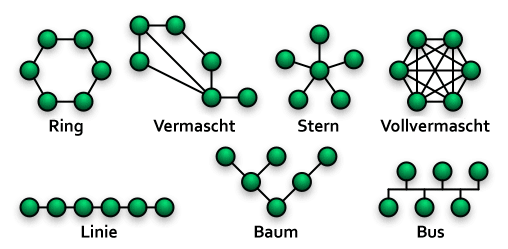
\includegraphics[width=0.5\textwidth]{images/netzwerkarten.png}
\end{figure}

\subsection{LVDS}
LVDS definiert kein Übertragungsprotokoll sondern eine Übertragungsart.
\begin{multicols}{2}
     \begin{figure}[H]
        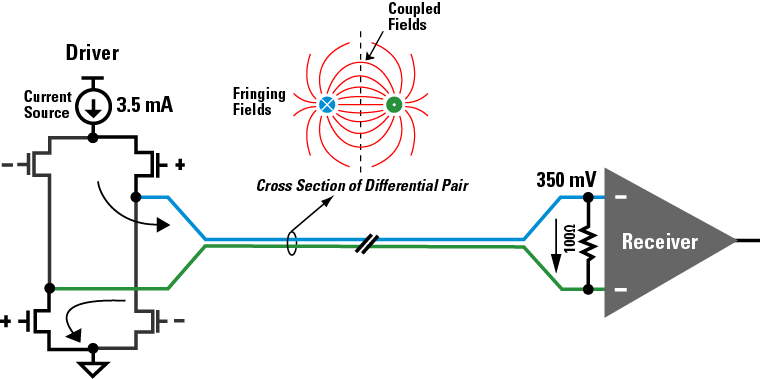
\includegraphics[width=0.5\textwidth]{images/lvds.png}
    \end{figure}

    \subsubsection{Prinzip}
    Die Signale werden anstelle mit einer Spannungsänderung mit einer Stromänderung übertragen. Das Signal schwingt somit nur um eine Spannung von $\pm$350mV.

    \subsubsection{Implementierung in VHDL}
    In VHDL kann LVDS nicht direkt synthetisiert werden. Der FPGA hat jedoch dennoch Pads, welche LVDS unterstützen. Diese müssen jedoch mithilfe von Constraints zugewiesen werden.
    \lstinputlisting[language=tcl]{code/tcl/lvds.xdc}
\end{multicols}

\subsection{VHDL Components}
\begin{multicols}{2}
Es gibt generische VHDL-Komponenten die für Kommunikationsinterfaces verwendet werden können. Sie alle beschreiben Teile des data link layers.
% \begin{itemize}
%   \item Schieberegister
%   \item RAM/ROM
%   \item FIFO Buffer
% \end{itemize}
\vfill\null
\columnbreak
\begin{figure}[H]
  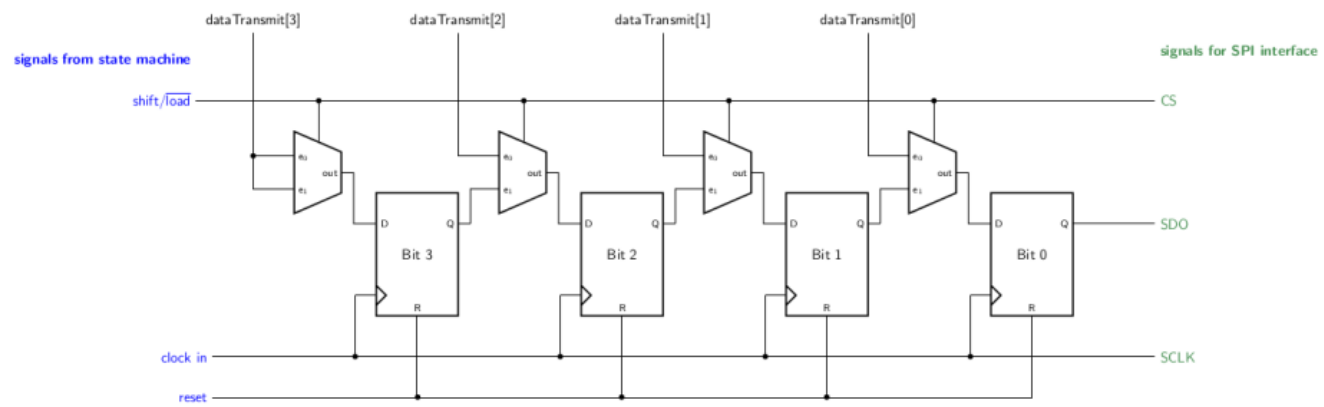
\includegraphics[width=0.5\textwidth]{images/shiftRegister.png}
\end{figure}
\end{multicols}

\section{Serial Communication Interfaces}
\subsection{SPI (Serial Peripheral Interface)}
In einem SPI Netzwerk kann jeweils nur ein Master vorhanden sein. Jedoch ist es möglich, dass mehrere Slaves am selben Bus angeschlossen sind. Die folgenden Signale werden für die SPI Schnittstelle benötigt:
\begin{compactitem}
    \item \textbf{SCLK}: Taktsignal
    \item \textbf{MOSI / SDO}: Datensignal vom Master zum Slave.
    \item \textbf{MISO / SDI}: Datensignal vom Slave zum Master.
    \item \textbf{CS}: Signalisiert dem Slave eine aktive Kommunikation. Sind mehrere Slaves am selben Bus angeschlossen, so existiert oft für jeden Slave ein eigenes CS-Signal.
\end{compactitem}

\subsubsection{Taktpolarität und Taktphase}
Es gibt insgesamt vier SPI-Modi. Diese unterscheiden sich in der Taktpolarität und Taktphase.
\begin{figure}[H]
    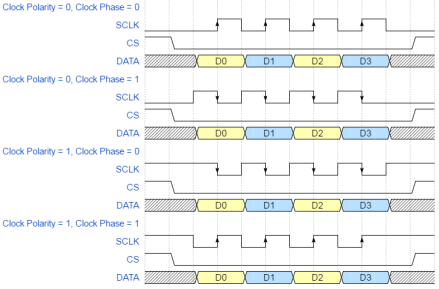
\includegraphics[width=0.5\textwidth]{images/spi_taktphase.png}
\end{figure}

\subsubsection{Timing}
Eine mögliche SPI Transaktion ist untenstehend zu sehen:
\begin{figure}[H]
    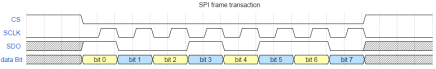
\includegraphics[width=1\textwidth]{images/spi_timing.png}
\end{figure}

\subsubsection{Hardwaremässige Implementierung}
Die Hardware für eine SPI Schnittstelle kann mittels zwei Schieberegistern (eines für das Senden, sowie eines für das Empfangen) realisiert werden.
\begin{multicols}{2}
    \begin{figure}[H]
        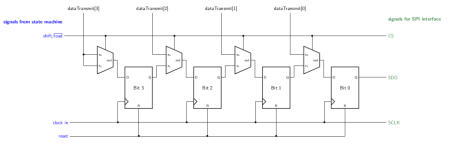
\includegraphics[width=0.5\textwidth]{images/spi_shift1.png}
    \end{figure}
    \begin{figure}[H]
        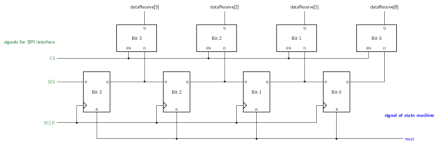
\includegraphics[width=0.5\textwidth]{images/spi_shift2.png}
    \end{figure}
\end{multicols}

\subsubsection{Implementierung in VHDL}
\lstinputlisting[language=VHDL]{code/spiMaster.vhd}

\subsection{I\textsuperscript{2}C (Inter-Integrated Circuit)}
Das I\textsuperscript{2}C Interface ist ein bidirektionales Bussystem. Es können beliebig viele Master und Slaves angehängt werden. Die folgenden Signale werden für die I\textsuperscript{2}C Schnittstelle benötigt:
\begin{compactitem}
    \item \textbf{SCL}: Taktsignal
    \item \textbf{SDA}: Bidirektionales Datensignal
\end{compactitem}

\subsubsection{Übertragungsgeschwindigkeiten}
Die folgenden Geschwindigkeiten sind im I\textsuperscript{2}C Standard definiert:
\begin{compactitem}
    \item standard mode: 100 kbit/s
    \item fast-mode: 400 kbit/s
    \item fast-mode-plus: 1 Mbit/s
    \item high-speed mode: 3.4 Mbit/s
\end{compactitem}

\subsubsection{Timing}
Die folgenden Zustände auf dem I\textsuperscript{2}C Bus sind möglich:
\begin{figure}[H]
    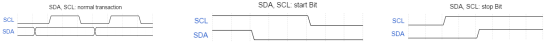
\includegraphics[width=1\textwidth]{images/i2c_bitstates.png}
\end{figure}
Eine mögliche I\textsuperscript{2}C Transaktion ist untenstehend zu sehen:
\begin{figure}[H]
    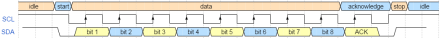
\includegraphics[width=1\textwidth]{images/i2c_timing.png}
\end{figure}
Nach dem Senden des Acknowledge-Bits, kann jeweils ein weiteres Byte gesendet werden, ohne die Transaktion durch Senden eines Stopbits zu unterbrechen. \\
Sollte ein Slave mehr Zeit brauchen um Daten zu verarbeiten, so kann er das SCL Signal auf Low ziehen, bis er wieder bereit ist.

\subsubsection{Arbitration}
Da mehrere Master und Slaves gleichzeitig senden könnten, ist eine Arbitrierung notwendig. Diese ist untenstehend dargestellt.
\begin{figure}[H]
    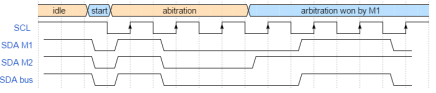
\includegraphics[width=0.75\textwidth]{images/i2c_arbitration.png}
\end{figure}
Der letzte Teilnehmer, welcher die SDA Leitung auf Low ziehen kann, gewinnt die Kommunikation.

\begin{multicols}{2}
    \subsubsection{Kommunikations Protokoll}
    \paragraph{Schreiben vom Master zum Slave}
    \begin{figure}[H]
        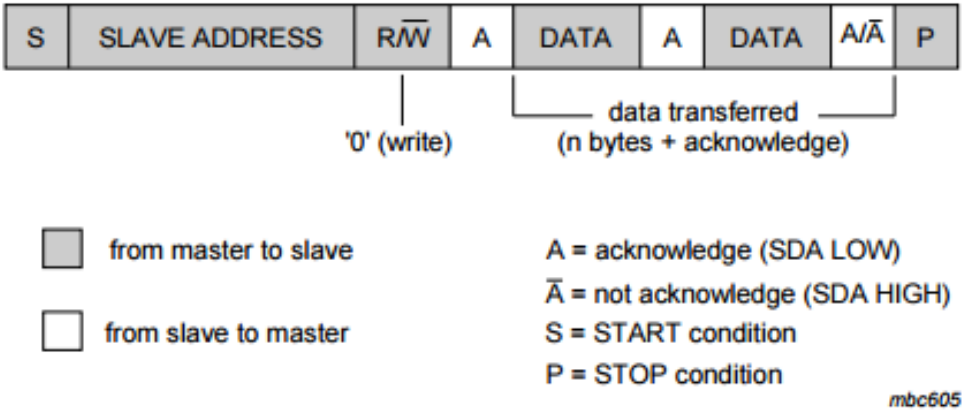
\includegraphics[width=0.5\textwidth]{images/i2c_protocolWrite.png}
    \end{figure}

    \paragraph{Lesen vom Slave}
    \begin{figure}[H]
        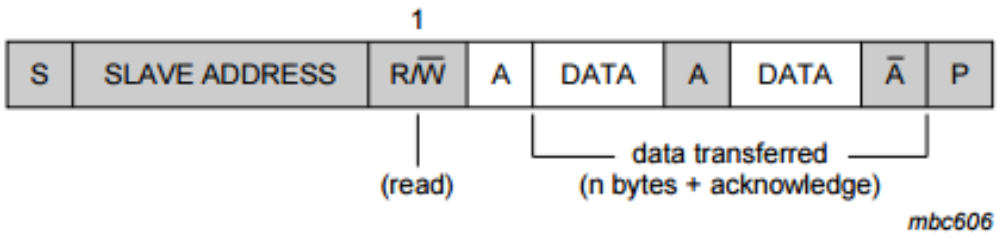
\includegraphics[width=0.5\textwidth]{images/i2c_protocolRead.png}
    \end{figure}

    \ \\ \ \\

    \subsubsection{Hardwaremässige Implementierung}
    Damit keine Kurzschlüsse entstehen, wenn zwei Master gleichzeitig senden wollen, werden die beiden Signale über externe Pull-Up-Widerstände auf einen High Pegel gezogen.
    \begin{figure}[H]
        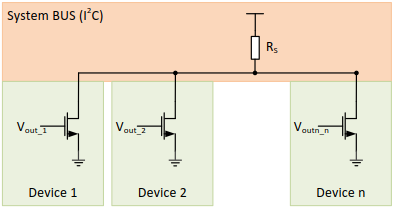
\includegraphics[width=0.5\textwidth]{images/i2c_hardware.png}
    \end{figure}
\end{multicols}

\subsubsection{Implementierung in VHDL}
Da die beiden I\textsuperscript{2}C-Signale bidirektional sind, muss in VHDL ein IO-Buffer für die beiden Signale instantiiert werden. Der nachfolgende Code instantiiert zwei solche Buffer.
\lstinputlisting[language=VHDL]{code/i2cMaster.vhd}

\subsection{UART (Universal Asynchronous Receiver Transmitter)}
UART ist eine Punkt-zu-Punkt Schnittstelle. Es wird pro Richtung ein Datensignal benötigt.

\subsubsection{Timing}
Eine UART Transaktion startet immer mit einem Startbit. Anschliessend wird ein Datenbyte gesendet, eine Parität, sowie ein Stoppbit (oder mehrere Stopbits). Da kein Takt mitgesendet wird, muss im Sender und Empfänger die Geschwindigkeit bekannt sein.
\begin{figure}[H]
    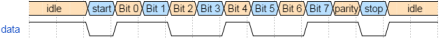
\includegraphics[width=0.75\textwidth]{images/uart_timing.png}
\end{figure}

\subsubsection{Hardwaremässige Implementierung}
\begin{figure}[H]
    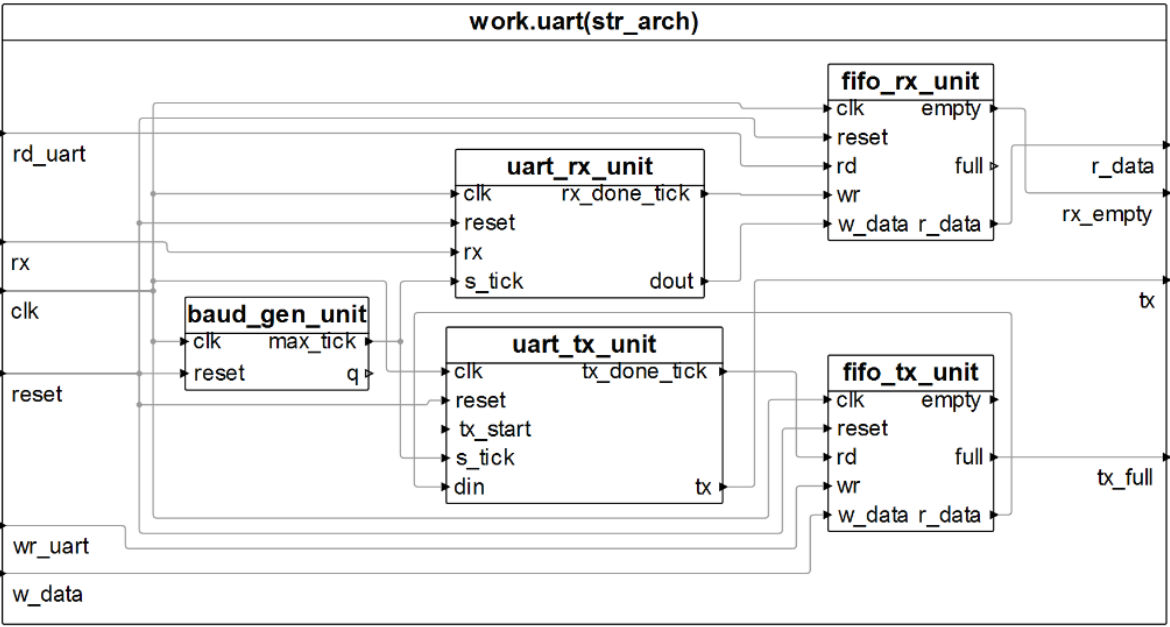
\includegraphics[width=0.75\textwidth]{images/uart_hardware.png}
\end{figure}

\subsubsection{VHDL Implementation}
\lstinputlisting[language=VHDL]{code/uart.vhd}

\section{Parallel Communication Interfaces}
\subsection{Vorteile paralleler Kommunikation}
\begin{compactitem}
    \item Parallele Kommunikation hat theoretischen Vorteil eines Durchsatzes, der N-mal grösser für eine N-Bit breite Kommunikation ist (gegenüber seriell).
    \item Parallele Kommunikation hat zusätzlichen Vorteil, dass keine Serialisierung / De-Serialisierung an Quelle und Senke benötigt wird $\rightarrow$ reduziert Hardwarekosten und Komplexität
\end{compactitem}

\subsection{Nachteile paralleler Kommunikation}
\begin{compactitem}
    \item In der Praxis stimmt die Aussage des Durchsatzes nicht. Clock und Data Skew bewirken, dass die Kommunikationsgeschwindigkeit der Geschwindigkeit des langsamsten Bits entspricht.
    \item Crosstalk zwischen den Leitungen ist ein weiteres Problem der parallelen Kommunikation. Parallele Datenleitungen beeinflussen sich gegenseitig und dadurch kann sich die Bitfehlerrate leicht erhöhen.
    \item Mit zunehmender Systemgröße von SoC-Komponenten hat die Anzahl der IOs ein Niveau erreicht, in dem die parallele Kommunikation mit der grossen Anzahl von benötigten IOs für die Off-Chip-Kommunikation mehr und mehr unwirtschaftlich wird $\rightarrow$ IOs verbrauchen Chipfläche und erzeugen somit Kosten.
\end{compactitem}

\subsection{AXI - Advanced eXtensible Interface}$~$ \\
Das AXI-Protokoll ist für eine hohe Bandbreite sowie eine kleine Latenzzeit ausgelegt. Es werden getrennte Lese- und Schreibbusse unterstützt. Weiter sind getrennte Busse für die Adressen sowie die Steuersignale vorhanden. Zusätzlich können auch sogenannte Burst-Transaktionen durchgeführt werden.

\subsubsection{Bustopologie und Modes}
Die AXI-Schnittstelle ist eine Multiple-Master-Multiple-Slave-Schnittstelle. Diese Topologie erfordert eine physikalische Verbindungsstruktur, die jeden Master mit jedem Slave verbindet. Die Topologie erlaubt es, dass zwei Master gleichzeitig Daten übertragen. Um Kollisionen zu vermeiden, ist ein Arbiter erforderlich, der entscheidet, welcher Master Zugriff auf einen Slave erhält. Es gibt verschiedene Verfahren, wie z. B. round-robin, preemptive priority, non-preemptive priority...
Der Lese- und Schreibkanal des Adressbusses kann geteilt werden, um Platz zu sparen. Dasselbe gilt auch für den Datenbus. Im AXI-Protokoll, müssen zwei Teile unterschieden werden:
\begin{compactitem}
  \item AXI interface ist eine 1-zu-1 Verbindung mit 5 unabhängigen Kanälen für Schreib-/Lesetransaktionen. Das AXI interface verbindet immer einen Master mit einer Slave-Node.
  \item AXI interconnect verbindet N Master mit N Slave Nodes. Es ist ein Logikblock, bestehend aus Arbitern, Multiplexern, Pipeline-Registern, vielen Verbindungen, einigen FIFOs und anderer Logik-Primitiven. AXI interconnect arbeitet als Switchbox um Signale von einer Master zu einer Slave-Node zu routen.
\end{compactitem}

\subsubsection{Kanäle}
\begin{multicols}{2}
    \begin{figure}[H]
     	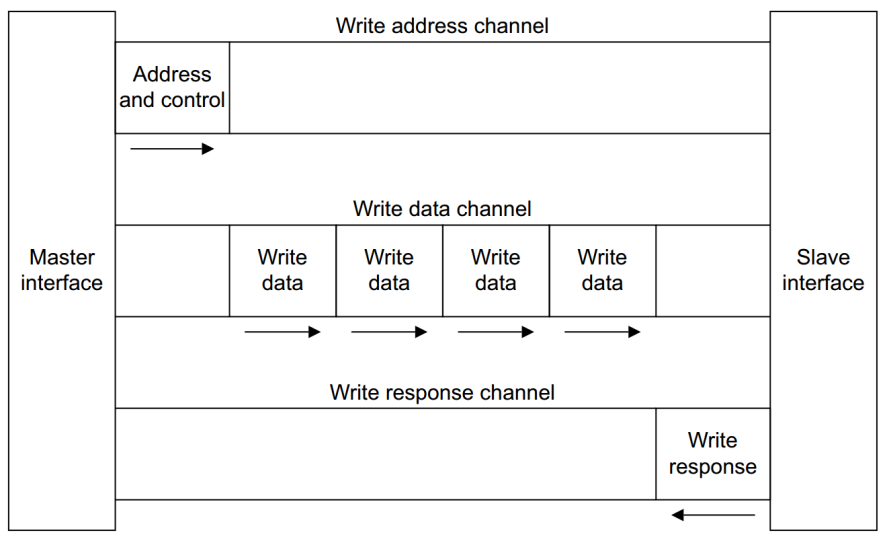
\includegraphics[width=0.4\textwidth]{images/AXI_Write_Data_Channels.png}
     \end{figure}
     \begin{figure}[H]
     	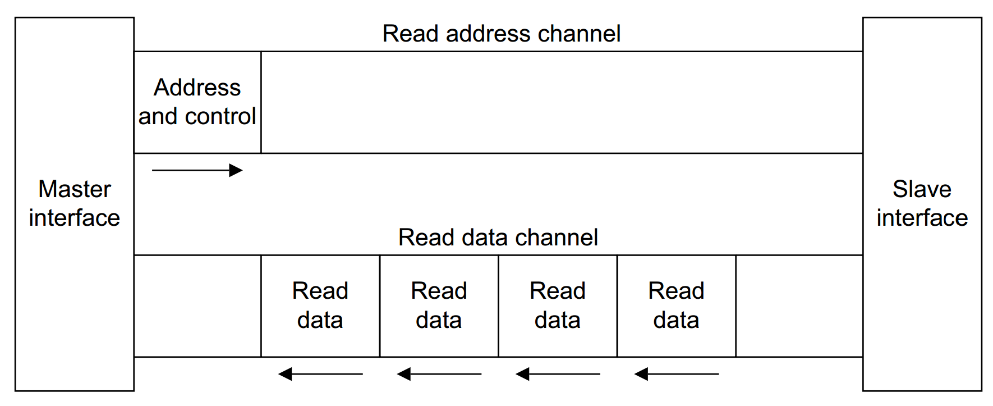
\includegraphics[width=0.5\textwidth]{images/AXI_Read_Data_Channels.png}
     \end{figure}
\end{multicols}
\begin{multicols}{2}
    \begin{compactitem}
        \item AW (write address channel) $\rightarrow$ Master zu Slave
        \item W (write data channel) $\rightarrow$ Master zu Slave
        \item WR (B) (write response channel) $\rightarrow$ Slave zu Master
        \item AR (read address channel) $\rightarrow$ Master zu Slave
        \item R (read data channel) $\rightarrow$ Slave zu Master
    \end{compactitem}
\end{multicols}

\begin{multicols}{2}
    \subsubsection{Handshaking}
    Für jeden Übertragungskanal existiert ein Handshaking. Ein Vorteil dieser Funktionsweise besteht darin, dass der Empfänger sowie der Sender die Geschwindigkeit der Datenübertragung steuern können.
     \begin{figure}[H]
     	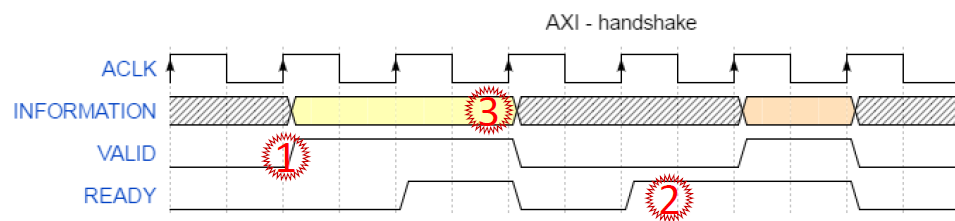
\includegraphics[width=0.5\textwidth]{images/AXI_Handshaking.png}
     \end{figure}
\end{multicols}
\begin{compactenum}
    \item Der Datensender setzt das Valid Signal, um anzuzeigen, dass Informationen verfügbar sind.
    \item Der Datenempfänger setzt das Ready Signal, um anzuzeigen, dass die Information akzeptiert werden kann.
    \item Eine Übertragung von Daten tritt auf, wenn sowohl das Valid als auch das Ready Signal an einer Taktflanke high sind.
\end{compactenum}

\begin{multicols}{2}
    \begin{figure}[H]
     	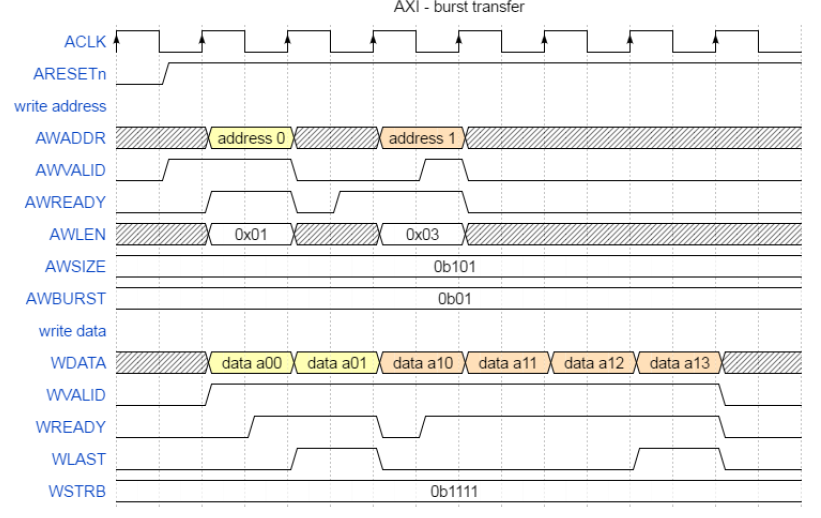
\includegraphics[width=0.5\textwidth]{images/AXI_Burst_Transfer.png}
     \end{figure}
    \paragraph{Burst Mode}$~$ \\
    Anstatt ein einziges Wort oder Byte in einer Transaktion zu senden, wird  im Burst-Modus ein gesamter Block von Daten gesendet. Dies ist sehr nützlich bei der Übertragung grosser Datenmengen.
\end{multicols}

\subsubsection{Varianten}
\begin{compactitem}
    \item AXI 4: Maximale Performance. Burst-Modus bis zu 256 Zyklen pro Adresse. Für Hochleistungsdatenaustausch.
    \item AXI-Lite: Vereinfachte Version von AXI 4. Für speicherabgebildete Einzeltransaktionen. Kein Burst. Für kleinen Datendurchsatz wie Austausch von Steuerungseinstellungen.
    \item AXI-Stream: Für High-Speed-Streaming. Keine Adressphase (nicht speicherzugeordnet). Unbegrenzte Datenburstgrösse. Daten vom Master zum Slave.
\end{compactitem}

\begin{multicols}{2}
\subsubsection{AXI Interconnect Block}
Für den Anschluss des AXI-Bussystems werden viele Interconnect Blöcke verwendet.
\begin{compactitem}
    \item Agiert als Slave vom PS
    \item Dient als Master für die Signalweiterleitung vom PS zu verschiedenen AXI-IP-Instanzen (Slaves).
    \item Unterstützt auch eine Protokollkonvertierung (z.b. Verbindung von AXI 3 und AXI 4)
\end{compactitem}
\vfill\null
\columnbreak
\begin{figure}[H]
  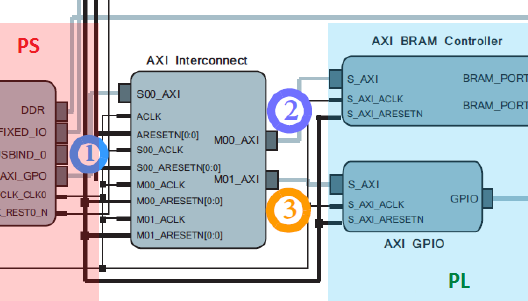
\includegraphics[width=0.5\textwidth]{images/AXI_Interconnect.png}
 \end{figure}
\end{multicols}
\begin{compactitem}
  \item SASD (Shared address bus and shared data buses) $\rightarrow$ Für weniger komplexe Systeme
  \item SAMD (Shared address bus and multiple data buses) $\rightarrow$ Durchsatz des Adressbusses ist kleiner als derjenige des Datenbusses, aufgrund der Burst-Fähigkeit des Datenkanals.
  \item MAMD (Multiple address bus and multiple data buses) $\rightarrow$ Für komplexe Systeme
\end{compactitem}

\subsubsection{Zynq: Processing System $\leftrightarrow$ Programmable Logic}
\begin{multicols}{2}
  Datenübertragung zwischen PS und PL erfolgt via AXI. Jede Schnittstelle realisiert einen kompletten AXI Bus. Insgesamt sind 9 AXI Schnittstellen vorhanden.
  \begin{figure}[H]
   	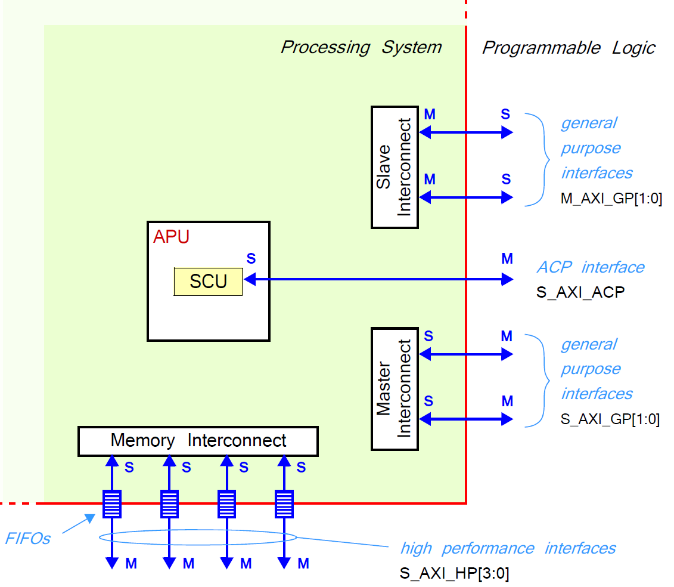
\includegraphics[width=0.5\textwidth]{images/AXI_PL_PS.png}
   \end{figure}
\end{multicols}

\section{Combining FPGA and Processor}
Oftmals erfolgt die Kommunikation zwischen PS und PL über AXI. Die meisten IPs aus dem IP-Katalog von Xilinx haben diese Schnittstelle implementiert.

\subsection{SDK}
Mit dem SDK von Xilinx kann der ARM Prozessor auf dem Zynq programmiert werden. Wird das SDK gestartet, so öffnet sich automatisch ein neues generiertes Beispielprojekt.

\subsubsection{Benutzen der AXI Schnittstelle}
Im Beispielprojekt wird eine Datei \textit{xparameters.h} erstellt. Diese enthält Definitionen über die vorhandenen AXI-Schnittstellen, wie zum Beispiel der Adressbereich. In der Datei \textit{xil\_io.h} sind Funktionen enthalten um Register über AXI zu lesen und zu schreiben. Das SDK erstellt zudem in der Datei \textit{AXILite.h} oder \textit{AXI.h} spezialisierte Funktionen, welche passend auf die über AXI angeschlossenen Komponenten zugeschnitten sind (es wird deshalb empfohlen die Funktionen aus diesen Dateien zu benutzen).
\lstinputlisting[language=C]{code/c/sdk_axi.c}

\subsubsection{AXI Direct Memory Access (DMA)}
Im IP Katalog von Xilinx gibt es einen AXI DMA IP Core. Dieser stellt zwei AXI4-Stream-Schnittstellen für eine hohe Bandbreite zur Verfügung. Eine Schnittstelle dient der Datenübertragung vom Master zum Slave, die andere für die gegengesetzte Richtung.

\begin{multicols}{2}
\paragraph{Verbindung mit ARM}
Um die beste  Performanz zu erreichen, sollte der IP Block wie nachfolgend dargestellt mit dem ARM verbunden werden:
\begin{figure}[H]
    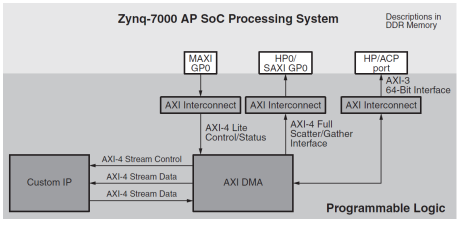
\includegraphics[width=0.5\textwidth]{images/sdk_dmaip.png}
\end{figure}

\paragraph{Modi}
Die folgenden Modi stellt der DMA IP Block zur Verfügung:
\begin{compactitem}
    \item \textbf{Register Direct Mode}: Dieser Modus wird benutzt, wenn eine hohe Geschwindigkeit zu einem Block im PL gefordert ist. Alle DMA Transfers werden gestartet, indem dem DMA-Blcok eine Ziel- oder Startadresse sowie eine Länge mitgeteilt wird. Sobald der Transfer abgeschlossen wurde, wird ein Interrupt generiert.
    \item \textbf{Scatter/Gatter Mode}: In diesem Mode werden Daten direkt in einen Speicher geschrieben, ohne dass vorher spezifisch eine Anforderung getätigt werden muss (benötigt mehr FPGA Ressourcen).
\end{compactitem}
\end{multicols}
\subsubsection{PL330 DMA}
Der Zynq stellt im PS einen eigenen DMA-Controller zur Verfügung. Bis zu acht Streams können von diesem Block gemanaged werden. Das SDK stellt in der Datei \textit{xdmaps.h} verschiedene Funktionen zur Ansteuerung des DMA-Controllers zur Verfügung.

\paragraph{DMA Schreibtransfer}
\lstinputlisting[language=C]{code/c/sdk_dmawrite.c}

\paragraph{DMA Lesetransfer}
\lstinputlisting[language=C]{code/c/sdk_dmaread.c}

%\section{Verifikation}$~$ \\
Oft wird die Verifikation als letzter Schritt nach dem Design bezeichnet. Doch die Verifikation beginnt viel früher und sie ist mehr als nur der Beweis der funktionalen Korrektheit. Sie beginnt auf Anforderungsebene und ist ein konstanter Prozess, der parallel zum Designprozess läuft.
\begin{compactitem}
    \item Verifikation bei Spezifikation: Ist das was ich möchte wirklich das was ich benötige?
    \item Verifikation beim Design: Habe ich tatsächlich das entwickelt, was gefordert wurde?
    \item Verifikation beim Testen: Kann ich defekte von fehlerhaften Schaltungen unterscheiden?
\end{compactitem}
Verschiedener Quellen zufolge wird deutlich, dass der Gesamtaufwand für die Verifikation mehr als 50\% des gesamten Entwicklungsaufwands beträgt - Tendenz wachsend!

\subsection{Dynamische Verifikationsmethoden}$~$ \\
Überprüft das Eingangs-/Ausgangsverhalten einer Schaltung. Eine Schaltung mit k Zuständen s und n Eingängen x wird durch ihre Zustandstabelle repräsentiert. Der Ausgang ist definiert durch: $y=f(x,s)$. Eine Möglichkeit dieser Verifikation wäre, bei jeder möglichen Kombination von x und s den Ausgang zu prüfen (Exhaustive Verification). In der Praxis ist dies nur für kleine Schaltkreise möglich, da die Anzahl der Testfälle schnell gegen Unendlich anwachst. Ein realistischer Kompromiss ist erforderlich, um viele potenzielle Fehler mit vernünftigem Aufwand zu finden. Eine Kombination folgender Methoden ist von Vorteil:
\begin{compactitem}
    \item Anwenden der assertion-basierten Verifikation
    \item Sammeln von Testfällen aus mehreren Quellen
    \item Arbeitskräfte in zwei unabhängige Teams für Schaltungsentwurf und Testdesign einteilen.
    \item Rapid Prototyping (schnelles und frühes Erstellen von Prototypen)
\end{compactitem}

\subsubsection{Assertion-basierte Verifikation}
Assertions sind kleine Codefragmente, die in den regulären Code eingebaut werden. Diese Fragmente fungieren als In-Code-Sanity-Checks. Sie sind nicht für die Synthese gedacht. Synthesizer können die meisten dieser Aussagen automatisch ignorieren.
Assertions müssen unerwartete Bedingungen bereits vor dem Debuggen überprüfen. Solche Bedingungen sind z.B.:
\begin{compactitem}
    \item Speicheradressen ausserhalb des erlaubten Bereichs
    \item Eintretende Fehlerzustände in Zustandsmaschinen
    \item Unvorhergesehene Eingabewerte
    \item Numerischer Über-/Unterlauf
\end{compactitem}
\lstinputlisting[language=VHDL,style=VHDL]{code/assert.vhd}
In VHDL 2008:
\lstinputlisting[language=VHDL,style=VHDL]{code/assert2008.vhd}
Die assert-Anweisung testet eine Condition (boolesche Bedingung). Wenn diese falsch ist, wird der Report ausgegeben. Mit Severity gibt man den Typ der Meldung an (note, warning, error, failure).

\subsubsection{Auswahl von Testfällen}
Die Stimuli sollten mit Vorsicht angewendet werden. Nachfolgend eine Auflistung von einigen wichtigen Testfällen:
\begin{compactitem}
    \item Stimuli anwenden, welche die Standardfunktionalität der Schaltung widerspiegeln. $\rightarrow$ Typisch für den Designer: Man definiert Testfälle um zu beweisen, dass die Schaltung die erwartete Funktionalität zeigt.
    \item Stimuli anwenden, welche wahrscheinlich zu ungewöhnlichen arithmetischen Bedingungen führen (z.B. Unter-/Überlauf, Teilung durch sehr kleine Zahlen usw.).
    \item Stimuli anwenden, welche bekannte Ausnahmefälle im Kontrollfluss widerspiegeln.
    \item Stimuli anwenden, welche aus realen Dienstleistungen bestehen.
    \item Anwenden von zufällig ausgewählten Testfällen.
\end{compactitem}
Real-World-Daten und zufällige Testfälle können nur angewendet werden, wenn die erwartete Antwort auf zufällige Eingabedaten bekannt ist. Diese Methode fragt nach einem goldenen Referenzmodell, das die erwartete Antwort für Zufallsdaten erzeugt. Solche goldenen Referenzmodelle können bereits bestehende Schaltungen bei einer Schaltungsrekonstruktion sein, sie kann ein High-Level-Modell sein (z.B. Matlab oder Simulink-Darstellung einer Schaltung) oder eine als Rapid Prototype implementierte Hardware-Darstellung (z.B. als SoC Direkt mit HLS oder System Generator synthetisiert).

\subsection{Simulation}$~$ \\
Für kleine Block Level Verifikationen genügt eine kleine Testbench in VHDL. Für grössere Schaltungen ist jedoch ein allgemeiner Ansatz erforderlich. Stimuli und erwartete Response werden als Eingabe- und Ausgabevektoren in einer Datei angegeben. Mittels read-Funktion (im TEXTIO Package) wird Zeile für Zeile eingelesen, mit den tatsächlichen Signalen verglichen und überprüft. Bei einer Nicht-Übereinstimmung erscheint während der Simulation eine dementsprechende Konsolenmeldung. In einem synchronen Design muss ein fester Zeitplan für Stimuli und Response eingehalten werden. Dieser regelmässige Zeitplan muss daher den folgenden Regeln entsprechen:
\begin{compactitem}
    \item Für jeden Testfall ein periodisches Taktsignal angeben
    \item Pro Taktzyklus ein Stimulus/Response-Paar verwenden
    \item Ein streng regelmässiges Muster für Stimuli/Response anwenden
\end{compactitem}
Automatisierte Test-Prozedur:
\lstinputlisting[language=VHDL,style=VHDL]{code/Automated_test_procedure.vhd}
Die Simulation kann in verschiedenen Designebenen durchgeführt werden:
\begin{multicols}{3}
    \begin{compactitem}
        \item Behavioral Simulation
        \begin{compactitem}
            \item Wird auf Stufe HDL durchgeführt $\rightarrow$ schnell
            \item Verifiziert nur die Funktionalität
            \item Es werden keine Timing-Informationen berücksichtigt
        \end{compactitem}
        \item Post Synthesis Simulation
        \begin{compactitem}
            \item Strukturelle Simulation
            \item Verifiziert die synthetisierte Netzliste
            \item Timing möglich, jedoch ungewöhnlich (da kein Routing) \ \\
        \end{compactitem}
        \item Post Implementation Simulation
        \begin{compactitem}
            \item Funktionelle und Timing Simulation möglich
            \item Präziseste, jedoch langsamste
        \end{compactitem} \ \\
    \end{compactitem}
\end{multicols}

\subsection{Debugging}$~$ \\
Die Simulation weist zwar auf ein Fehlverhalten der Schaltung hin, zeigt jedoch nicht die genaue Ursache. Das Lokalisieren eines Fehlers nennt man Debugging.\\
Es gibt zwei (bzw. drei) Bedingungen für das Finden von Fehlern:
\begin{compactitem}
    \item Fehlersensibilisierung (bug sensitization): Stimuli müssen die Knoten auf die invertierten logischen Werte treiben können um einen Bug an einem bestimmten Knoten ausfindig machen zu können.
    \item Fehlerfortpflanzung und Beobachtung (bug propagation and observation): Ein falscher Logikwert an einem Knoten muss beobachtbar sein oder er muss zumindest an einen Knoten weitergegeben werden können, der beobachtbar ist.
\end{compactitem}

\subsubsection{Simulationswerkzeuge}
Mit purer Input/Output Simulation kann man die obigen Bedingungen nicht erfüllen. Spezielle Simulationswerkzeuge bieten jedoch perfekte Beobachtbarkeit, mit welchen alle internen Knoten beobachtet werden können. Auch bei der Sensibilisierung dienen diese Simulationswerkzeuge perfekt: Während eine Testbench nur die Eingänge einer zu prüfenden Schaltung ansteuern kann, können hier interne Knoten direkt durch Erzwingen von Signalen auf einen festen Wert angesteuert werden.

\subsubsection{Emulation}
Während bei der Simulation beinahe das ganze Spektrum der Debuggingtools verwendet werden kann, sind Fehler bei der Emulation viel schwieriger zu finden. Es gibt fast keine Möglichkeit, interne Knoten von integrierten Schaltungen beobachten zu können. Aufgrund der umprogrammierbaren Struktur eines FPGA ist jeder Schaltungsknoten inhärent zu beobachten und kann inhärent stimuliert werden. Dies geschieht über die eingebaute JTAG-Schnittstelle. XILINX stellt zwei spezielle Blöcke zur Verfügung:

\paragraph{Virtual input and output (VIO)}$~$ \\
Interne Knoten können als Ein- oder Ausgänge definiert werden. Der Mechanismus funktioniert über die JTAG-Schnittstelle. VIO Blöcke sind Hardwarekomponenten. Sie müssen in den Code integriert werden. Anschliessend werden sie instanziiert, synthetisiert und schliesslich implementiert. Die neu generierten Ein- und Ausgänge des VIO können während der Debug-Session getrieben und analysiert werden.

\paragraph{Integrated Logic Analyzer (ILA)}$~$ \\
ILA dient zur Überwachung interner programmierbarer Logiksignale für die Nachanalyse. ILA Blöcke bieten mehrere konfigurierbare Triggereinheiten und bis zu 64 konfigurierbare Sonden für die Analyse in einer GUI-Darstellung. ILA bietet auch Cross-Trigger-Funktionalität zwischen dem ARM-Prozessor und dem logic fabric part.
%NOTE: nicht Prüfungsinhalt für HS19
\section{Verification Design For Test}
\subsection{Warum testen?}$~$ \\
In der Fabrikation von elektronischen Systemen gibt es unzählige Fehlerquellen. Je früher ein Fehler erkennt werden kann, desto weniger teuer kommt er zu stehen. Eine Regel besagt, dass die Kosten mit jedem Produktionsschritt, bei welchem der Fehler nicht erkannt wurde, um den Faktor 10 ansteigen. Bei der Herstellung von digitalen Chips kann in der Regel mit einer Ausbeute von 95 bis 98\% gerechnet werden.

\subsection{Begriffe}
\begin{description}
  \item[Defect] Physikalische Fehlerquelle in integrierten Schaltungen
  \item[Fault] Messbare Fehlfunktion einer Schaltung aufgrund von einem/mehreren Fehler(n)
  \item[Quality] Mass für die exakte Erfüllung der Vorgaben (4 Bereiche: Design-, Herstellungs-, Auslieferungs- und Betriebsqualität)
  \item[Yield] Verhältnis von funktionierenden Teilen auf einem Wafer: $y_f = \frac{\#good\_circuits}{\#manufactured\_circuits}$
  \item[Defect level] Anteil an nicht-funktionierenden Chips, die unerkannt bleiben: $D_L = \frac{\#defective\_sold}{\#total\_sold} = 1 - y_f^{1-F_c}$
  \item[Fault coverage] Anteil an Fehlern die mit einem Set von Testvektoren erkannt werden können: $F_c = \frac{\#detectable\_Faults}{\#possible\_Fault}$
\end{description}


\subsection{Fehlermodelle}$~$ \\
Die nachfolgenden Fehlermodelle gibt es:
\begin{compactitem}
    \item \textbf{Stuck-At-0-Fault / Stuck-At-1-Fault}: Das entsprechende Signal wird auf einem Low-Pegel (Stuck-At-0-Fault) oder auf einem High-Pegel (Stuck-At-1-Fault) festgehalten und kann sich nicht ändern.
    \item \textbf{Bridging-Fault}: Bezeichnet einen Kurzschluss zwischen zwei Signalen. Ein Kurzschluss nach VDD oder VSS äussert sich wie ein Stuck-At-X-Fault. Ein Kurzschluss zwischen zwei Signalleitungen, verhält sich wie ein OR oder AND und kann im besten Fall funktional nachgewiesen werden.
    \item \textbf{Delay-Fault}: Dies sind eigentlich keine funktionalen Fehler, sondern Fehler in der Verzögerungszeit, hervorgerufen durch zu hohe Widerstandswerte der Verbindungen. Sie äussern sich letztlich jedoch funktional.
\end{compactitem}

\subsection{Fehlererkennung}
\subsubsection{Detektion von Stuck-At-X-Fault}
Um einen solchen Fehler zu detektieren, muss der entsprechende Knoten kontrollier- und beobachtbar sein. Kontrollierbar ist er dann, wenn er über ein externes Signal auf Low oder High gesetzt werden kann. Beobachtbar ist er dann, wenn sein Zustand von aussen überprüft werden kann.
\paragraph{Beispiel}$~$ \\
Anhand untenstehender Schaltung, wird nun eine Tabelle mit allen Testvektoren erstellt. In der Y-Spalte steht der Ausgangswert, wenn kein Fehler vorhanden ist. In den nachfolgenden Spalten, steht der Ausgangswert wenn der entsprechende Stuck-At-Fehler vorhanden ist.\ \\
\begin{minipage}{0.6\textwidth}
\begin{figure}[H]
    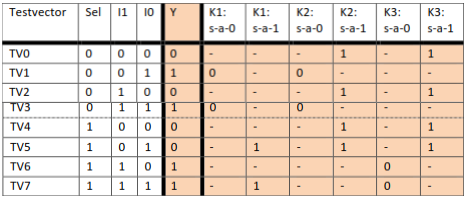
\includegraphics[width=1.0\textwidth]{images/stuckat_detektion_1.png}
\end{figure}
\end{minipage}
\hfill
\begin{minipage}{0.35\textwidth}
\begin{figure}[H]
    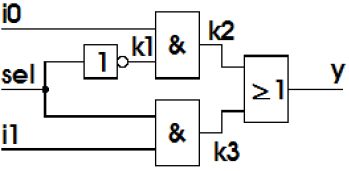
\includegraphics[width=1.0\textwidth]{images/stuckat_detektion_schaltung.png}
\end{figure}
\end{minipage} \\
Nun soll anhand der erstellten Tabelle, die Testvektorenanzahl auf ein Minimum beschränkt werden (Fault Collapsing). Mit den Testvektoren TV1, TV5 und TV7 kann somit jeder Fehler detektiert werden.
\begin{figure}[H]
    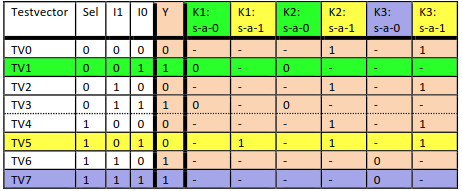
\includegraphics[width=0.6\textwidth]{images/stuckat_detektion_2.png}
\end{figure}

\subsubsection{Fehlerabdeckung (Fault coverage)}
Die Fehlerabdeckung kann folgendermassen berechnet werden: $\text{Fehlerabdeckung}=\frac{\text{Anzahl detektierter Fehler}}{\text{Abzahl möglicher Fehler}}*100\%$ Im Allgemeinen sollte darauf geachtet werden, dass eine Fehlerabdeckung von mindestens 95\% erreicht wird.

\subsubsection{Redundante Logik}
Sollte redundante Logik eingebaut sein (zur Verhinderung von Hazards), so kann die Funktion nicht ohne Zusatzaufwand getestet werden.
\paragraph{Beispiel}$~$ \\
Anhand von untenstehender Schaltung, wird die nachfolgende Tabelle erstellt. Dabei stellt sich heraus, dass ein Stuck-At-0-Fault am Knoten K4 nicht detektiert werden kann. Wenn aber die am Ausgang angeschlossene Logik darauf baut dass kein Hazard auftritt, kann dies zu einem Fehlverhalten führen.\\
\begin{minipage}{0.6\textwidth}
\begin{figure}[H]
    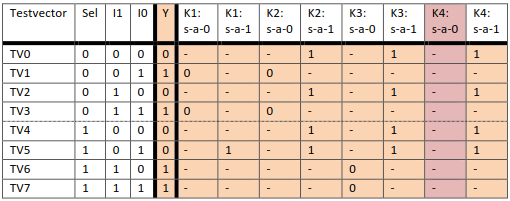
\includegraphics[width=1.0\textwidth]{images/stuckat_redundant_1.png}
\end{figure}
\end{minipage}
\hfill
\begin{minipage}{0.35\textwidth}
\begin{figure}[H]
    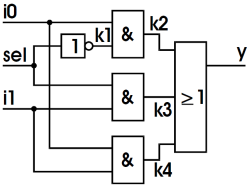
\includegraphics[width=1.0\textwidth]{images/stuckat_redundant_schaltung.png}
\end{figure}
\end{minipage}
\subsection{I\textsubscript{DDQ}-Test}$~$ \\
\begin{multicols}{2}
Beim I\textsubscript{DDQ}-Test wird die Ruhestromaufnahme der Schaltung gemessen. Dieser Ruhestrom ist im Normalfall vernachlässigbar klein. Entsteht jedoch bei einem Signalwert ein Kurzschluss, so ist dies über den Ruhestrom feststellbar. Wird bei einer Schaltung festgestellt, dass direkt nach dem Anlegen der Versorgungsspannung ein hoher Strom fliesst, kann auf nachfolgende Tests direkt verzichtet werden, was die Testzeit stark verkürzt.
\begin{figure}[H]
    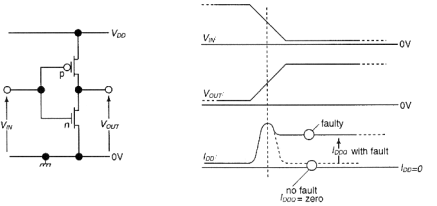
\includegraphics[width=0.5\textwidth]{images/iddq.png}
\end{figure}
\end{multicols}

\subsection{Scan Path}$~$ \\
Die Scan Path Methode adressiert das Problem, dass interne Knoten von aussen schlecht kontrollierbar und beobachtbar sind. Dazu wird vor jedes Flipflop ein 2:1 Multiplexer geschalten (Scan Flipflop), mit dessen Hilfe alle Flipflops zu einem riesigen Schieberegister zusammengeschaltet werden. \\
\begin{minipage}{0.25\textwidth}
\begin{figure}[H]
    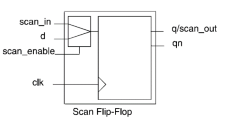
\includegraphics[width=1.0\textwidth]{images/scanflipflop.png}
\end{figure}
\end{minipage}
\hfill
\begin{minipage}{0.7\textwidth}
Die folgenden speziellen Signale sind nun vorhanden:
\begin{compactitem}
    \item \textit{scan\_enable}: Legt die Multiplexer Stellung fest.
    \item \textit{scan\_in}: Eingangssignal für das Schieberegister. Wird während dem Normalbetrieb nicht benötigt.
    \item \textit{scan\_out}: Ausgangssignal des Schieberegisters. Führt auf den \textit{scan\_in} Eingang des nächsten Flipflops.
\end{compactitem}
\end{minipage}

In einem ersten Schritt wird das ganze Schieberegister seriell befüllt. Damit können alle internen Eingänge kontrolliert werden. In einem zweiten Schritt wird das System für einen Taktzyklus in den Normalbetrieb versetzt. Im letzten Schritt wird das Schieberegister nun wieder seriell ausgelesen.

\subsubsection{Parallele Pfade}
Je mehr Flipflops sich in einem Design befinden, umso länger wird der Scan Pfad und somit auch die Testzeit. Durch die Verteilung der Flipflops auf mehrere Scan Pfade wird die Testdauer verkürzt. Es wird dabei versucht, die Scan Pfade möglichst auszubalancieren, damit es bei allen Pfaden gleich lange dauert um die Daten auszulesen oder zu schreiben.

\begin{multicols}{2}
    \subsubsection{Scan Path bei mehreren Taktdomänen}
    Sind in einem System unterschiedliche Taktdomänen vorhanden, so kommen Lock-Up Latches, an den Übergängen von einer Domäne zur anderen, zum Einsatz. Diese stellen sicher, dass keine laufzeitbedingten Fehler auftreten.

    \subsection{BIST (Built In Self Test)}$~$ \\
    Der Test von grossen programmierbaren Blöcken (z.B. RAM, ROM, PLA, ...) ist mit Scan Paths nur schwer möglich, da die Anzahl Testvektoren nicht wirklich reduziert werden kann, da auch wirklich jede Zelle überprüft werden muss. Aus diesem Grund wird jeder Makrozelle eine zusätzliche Logik zugeordnet, mit welcher diese einen Selbsttest durchführen kann. \ \\ \ \\
    \begin{figure}[H]
        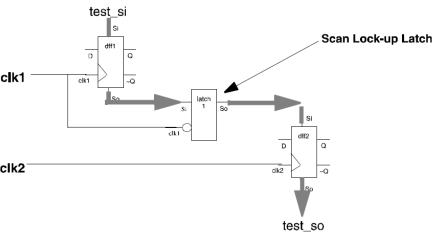
\includegraphics[width=0.5\textwidth]{images/scanpath_lookuplatch.png}
    \end{figure}
\end{multicols}

\subsubsection{Prinzip}
\begin{multicols}{2}
\begin{figure}[H]
    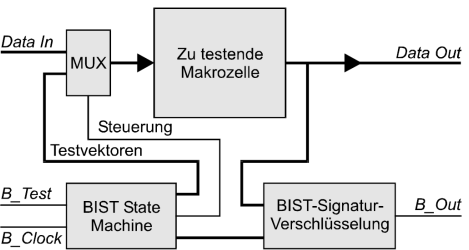
\includegraphics[width=0.5\textwidth]{images/prinzip_bist.png}
\end{figure}
Nebenstehend ist der prinzipielle Aufbau einer BIST-Zusatzlogik zu sehen. In den Eingangspfad der zu testenden Makrozelle ist ein 2:1-Multiplexer geschaltet. Über den Block BIST State Machine, der die Steuerlogik und einen Testmustergenerator enthält, wird dieser Multiplexer so geschaltet, dass entweder von aussen kommende Daten an die Makrozelle geführt werden (Normalbetrieb), oder solche vom Testmustergenerator (Testbetrieb). Die Ausgänge der Makrozelle werden neben der normalen Verdrahtung dem Block BIST-Signature-Verschlüsselung zugeführt. Dieser wertet die Testergebnisse aus und meldet sie nach aussen.
\end{multicols}
%NOTE: nicht Prüfungsinhalt für HS19
% \subsection{BST (Boundary Scan Test)}$~$ \\
% Die zunehmende Packungsdichte erschwert den Test von fertigen Baugruppen erheblich. Um die Anzahl erforderliche Prüfanschlüsse zu minimieren, wurde der BST entwickelt.
%
% \begin{multicols}{2}
%     \subsubsection{Konzept}
%     Jeder Ein- und Ausgang eines Chips wird mittels einer BSC (Boundary Scan Cell) vom Kern der Schaltung abgetrennt. Alle diese BSCs sind wiederum zu einem grossen Schieberegister zusammengeschalten (BSR - Boundary Scan Register).
%
%     \paragraph{Signale}$~$ \\
%     Jeder Chip stellt nach Aussen die folgenden Signale zur Verfügung, resp. benötigt die folgenden Signale:
%     \begin{compactitem}
%         \item \textit{TDI}, \textit{TDO}: Test Data In / Test Data Out, werden auf der Leiterplatte zu einem Schieberegister verknüpft. Sprich jeder TDO führt auf den TDI des nächsten Chips.
%         \item \textit{TCK}: Test Clock
%         \item \textit{TMS}: Test Mode Select
%         \item \textit{TRST*}: Optional, bringt den Chip in einen definierten Zustand
%     \end{compactitem}
%
%     \subsubsection{Realisierung auf dem Chip}
%     Jeder Chip muss für BST die folgenden Elemente beinhalten:
%     \begin{compactitem}
%         \item \textbf{Bypass-Register}: Überbrückt dass BSR. So kann der entsprechende IC bei gewissen Test übersprungen werden. Dies verkürzt wiederum die Testdauer.
%         \item \textbf{Device-ID-Register}: Enthält eine ID des Chips. Dieses Register kann während dem Test ausgelesen wertden um z.B. auf korrekte Bestückung zu prüfen.
%         \item \textbf{TAP (Test Access Port)}: Schnittstelle nach Aussen
%         \item \textbf{Instruction-Register}: Steuert die internen notwendigen Multiplexer Einstellungen.
%     \end{compactitem}
%     \begin{figure}[H]
%         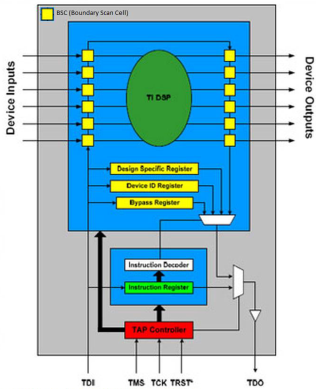
\includegraphics[width=0.5\textwidth]{images/bst_aufbau.png}
%     \end{figure} \ \\ \ \\
% \end{multicols}
%
% \begin{multicols}{2}
%     \subsubsection{TAP-Kontroller}
%     Die Funktion des TAP-Kontrollers ist in nebenstehender Grafik dargestellt. In den Zustand \textit{Test-Logic-Reset} wird gewechselt wenn das \textit{TRST*}-Signal gesetzt wird oder indem das Signal \textit{TMS} während fünf Taktzyklen auf einem High-Pegel gehalten wird.
%
%     \subsubsection{Instruktionen}
%     \paragraph{Instruktions-Register}
%     Das Instruktions-Register muss mindestens eine Länge von zwei Bit aufweisen um die verbindlichen Befehle dekodieren zu können. Das Register kann aber durchaus grösser sein, da viele Hersteller noch eigene Befehle implementieren. \\
%     Wenn der TAP-Kontroller sich im Zustand \textit{Shift\_IR} befindet, wird die Instruktion seriell vom Eingang \textit{TDI} in das Instruktions-Register geladen.
%
%     \begin{figure}[H]
%         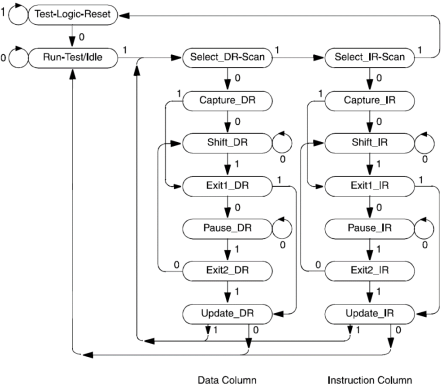
\includegraphics[width=0.5\textwidth]{images/bst_tapkontroller.png}
%     \end{figure}
% \end{multicols}
%
% \paragraph{Verbindliche Befehle}$~$ \\
% Die folgenden Befehle müssen in jedem Fall implementiert sein:
% \begin{compactitem}
%     \item \textbf{BYPASS}: Der Befehlscode besteht aus lauter Einsen (11...1). Ist dieser Befehl aktiv, muss im Zustand \textit{Shift\_DR} das Bypass-Register in den \textit{TDI}/\textit{TDO} Pfad geschaltet sein. Ebenfalls dürfen die Testregister die Kernlogik nicht beeinflussen.
%     \item \textbf{SAMPLE} / \textbf{RELOAD}: Nimmt eine Momentanaufnahme des aktuellen Zustandes der IC-Anschlüsse auf oder setzt die IC-Anschlüsse auf einen definierten Zustand. Das BSR wird im Zustand \textit{Shift\_DR} bei diesem Befehl in den \textit{TDI}/\textit{TDO} Pfad geschalten.
%     \item \textbf{EXTEST}: Der Befehlscode besteht aus lauter Nullen (00...0). Die Chiplogik wird bei diesem Befehl von der Leiterplatte isoliert (Die Kernlogik muss so abgeschottet sein, dass sie nicht beschädigt werden kann). Das BSR wird im Zustand \textit{Shift\_DR} bei diesem Befehl in den \textit{TDI}/\textit{TDO} Pfad geschalten.
% \end{compactitem}
%
% \paragraph{Interner Aufbau}$~$ \\
% Nachfolgend ist dargestellt, wie der TAP-Kontroller intern mit den vorhandenen Registern verschaltet ist.
% \begin{figure}[H]
%     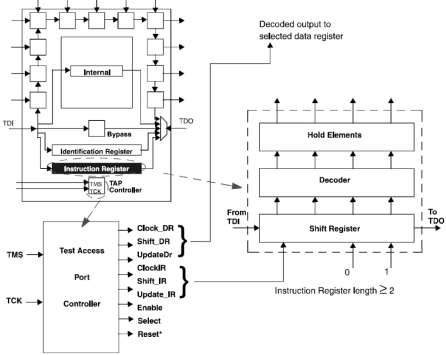
\includegraphics[width=0.75\textwidth]{images/bst_tapkontroller_verschaltung.png}
% \end{figure}
%
% \paragraph{Optionale Befehle}$~$ \\
% Die nachfolgenden Befehle sind optional, werden jedoch auch häufig implementiert:
% \begin{compactitem}
%     \item \textbf{INTEST}: Testet die Kernlogik eines Chips. Die Kernlogik wird zu diesem Zweck von den Ein- und Ausgängen isoliert.
%     \item \textbf{RUNBIST}: Startet einen eingebauten BIST-Selbsttest. Der Vorteil dieser Variante ist (im Gegensatz zum \textit{INTEST}) dass die Konfiguration des Chips nicht selber vorgenommen werden muss und am Schluss nur das Ergebnis überprüft werden muss.
%     \item \textbf{IDCODE}: Liefert den Inhalt aus dem Identifikations-Register zurück.
% \end{compactitem}
% \begin{multicols}{2}
% \subsubsection{Aufbau BYPASS-Register}
% \begin{figure}[H]
%     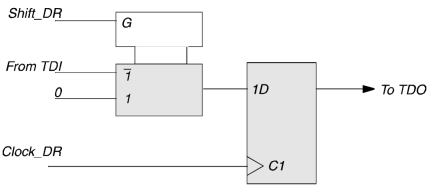
\includegraphics[width=0.5\textwidth]{images/bst_bypassregister.png}
% \end{figure}
%
% \subsubsection{Aufbau ID-Register}
% Das Identifikations-Register ist immer 32bit breit.
% \begin{compactitem}
%     \item \textbf{Bit 31-28}: Chip-Version
%     \item \textbf{Bit 27-12}: Frei verwendbar vom Hersteller
%     \item \textbf{Bit 11-1}: Standardisierter Hersteller Code
%     \item \textbf{Bit 0}: Immer 1
% \end{compactitem}
% \end{multicols}
% \subsubsection{Aufbau BSC}
% \begin{multicols}{2}
% \begin{figure}[H]
%     \includegraphics[width=0.5\textwidth]{images/bst_bsc.png}
% \end{figure}
% Für jeden Ein- und Ausgang eines Chips wird eine Zelle benötigt. Falls aber Three State-Ausgänge oder bidirektionale Anschlüsse vorkommen, dann muss auch deren Enable-Signal mit einer BSC versehen werden. Falls mehrere solcher Signale zu einem Bus zusammengefasst werden, dann werden alle entsprechenden Enable-Signale von derselben BSC geschaltet.
% \end{multicols}

%input{sections/11_HDL_Attributes}%NOTE: nicht Prüfungsinhalt für HS19
%\section{Digital Design For ASICS}
Moderne FPGA-Designs haben viel gemeinsam mit modernen ASIC-Designs. Trotzdem gibt es einige grundlegende Unterschiede.
\subsection{Zielanwendungen}
Im Vergleich zu FPGA-Designs sprechen die ASIC-Designs einen anderen Markt an. ASIC-Designs eignen sich in der Regel für Anwendungen mit hohem Produktionsvolumen, d.h. mindestens 100'000 Stücke pro Jahr, weil die NRE Kosten (einmalige Entwicklungskosten) sehr hoch sind. 
\paragraph{Gesamtkosten pro Einheit} 
$c=\frac{c_0}{n}+c_1$ \ \ \ c\textsubscript{0}: Summe der einmaligen Entwicklungskosten $\rightarrow$ konstant // n: Anzahl der entwickelten ASICS // c\textsubscript{1}: Kosteninkrement pro erzeugter Schaltung (für Rohwafer, Waferbearbeitung, Prüfung, Verpackung, Logistik usw.) $\rightarrow$ linear steigend
\begin{multicols}{2}
\textbf{c\textsubscript{0} ist ist abhängig von:} 
\begin{compactitem}
    \item Herstellungsprozess und Prozessoptionen, die die Masken- und die Waferherstellungskosten bestimmen
    \item Lizenzkosten und Lizenzgebühren für IP-Cores
    \item CAD-Tool-Kosten
    \item Engineering-Kosten für Design der Schaltung und Design der Testlösung
    \item Aufbau der Versorgungs- und Logistikkette
    \item etc.
\end{compactitem}
\textbf{c\textsubscript{1} ist abhängig von:} 
\begin{compactitem}
    \item Schaltungsgrösse
    \item Testzeit
    \item Herstellungsertrag
    \item Verpackungskosten
    \item etc.
\end{compactitem}
\ \\ \ \\
\end{multicols}
Beim FPGA-Design ist c\textsubscript{0} relativ klein im Vergleich zum ASIC-Design. Die Startkosten bei c\textsubscript{1} sind beim FPGA-Design tiefer als im ASIC-Design. Jedoch steigen die Kosten beim FPGA-Design steiler an als beim ASIC-Design. Der Schnittpunkt der beiden Gesamtkosten ergibt ungefähr Volumengrenze zwischen FPGA- und ASIC-Entwicklung. 
\subsection{Design Flow}
\begin{figure}[H]
    \includegraphics[width=1\textwidth]{images/ASIC_FPGA.png}
\end{figure}
\subsubsection{Synthese (FPGA vs. ASIC)}
\paragraph{FPGA}
\begin{compactitem}
    \item Target device bestimmen/auswählen (Hersteller, Familie, FPGA Typ)
    \item Wahl des Sythetisiertools
    \item Constraints hinzufügen (im XDC-Format) 
    \item Für kombinatorischen Teil werden LUTs und für den sequentiellen Teil FF erzeugt. 
    \item Hat Scankette eingebaut, da Scan und JTAG beim Programmieren gebraucht wird.
\end{compactitem}
\paragraph{ASIC}
\begin{compactitem}
    \item Wahl des Designhouse: ASIC-Design erfordert Wissen, Erfahrung und Infrastruktur, welche nicht immer vorhanden ist $\rightarrow$ evtl. Designhouse
    \item Wahl des Sythetisiertools (teuer!)
    \item Wahl der Technologie
    \item Wahl der digitalen Zellenbibliothek
    \begin{compactitem}
        \item High Density (9 or 10 tracks high): Mittlere Transistorgrösse für hohe Dichte und gute Performance, low power
        \item Ultra-High Density (7 or 8 tracks high): Kleine Transistorgrösse für sehr hohe Dichte und low power
        \item High Performance (12 tracks high): Grosse Transistorgrösse für optimale Geschwindigkeit, auch low power features
    \end{compactitem}
    \item Wahl der Soft- und Hard IP Blöcke (Block RAMs, DSP Blöcke, etc. sind normalerweise nicht vorhanden $\rightarrow$ kaufen
    \item Constraints hinzufügen (im SDC-Format) 
    \item Erzeugung generische Netzliste (im .edif Format), welche grundlegende boolesche Funktionen, die keine realen Gatter mit Layout und Timing sind, verwendet. Technologieunabhängig.
    \item Mapping, bei welchem die Grundfunktionen auf reale Zellen aus der Zellbibliothek abgebildet werden.
    \item Hat keine eingebauten Testfunktionen. Die Testlogik wird erzeugt und während der Synthese hinzugefügt $\rightarrow$ FFs werden durch Scan-FFs ersetzt. Scan-Kette wird erzeugt.
\end{compactitem}

\subsubsection{Floorplanning}
Floorplanning bezieht sich darauf, einzelne Elemente, Schaltungsblöcke und IOs vorläufig auf einem physikalischen Layout zu platzieren. Im FPGA-Design ist das Floorplanning ein Teil des Place and Route (Hinzufügen von Physical Constraints).

\subsubsection{Place and Route (FPGA vs. ASIC)}
\paragraph{FPGA}
\begin{compactitem}
        \item Zuweisung der verschiedenen Netzlistenelemente zu vorhandenen LUTs, FFs und Hardware-Makros auf dem FPGA-Chip $\rightarrow$ wird automatisch bei ''Run Implementation'' und ''Generating Bitstream'' zugewiesen. 
        \item Einfluss nur bedingt via Physical Constraints
\end{compactitem}
\paragraph{ASIC}
Besitzt mehrere Teilschritte:
\begin{compactitem}
        \item Power Planning: Generiert den Powerring, der VDD und VSS um den gesamten Chip erzeugt. Für horizontale Verbindungen und vertikale Verbindungen werden unterschiedliche Metallschichten verwendet.
        \item Definition Power Grid für Standardzellen: Abhängig von der ausgewählten Standardzellenbibliothek und ihrer charakteristischen Höhe wird das Gitter für VDD und VSS der Standardzellen erzeugt.
        \item Platzierung der Standardzellen (iterativer Prozess): Standardzellen werden mit einem bestimmten Dichtefaktor platziert, was bedeutet, dass ein gewisser Raum zwischen den Zellen frei bleibt. Dann versucht das Tool, die Leitungen zwischen den Zellen zu setzen. Wenn das Routing nicht erfolgreich war, startet der Prozess erneut mit einem neuen Placement. Wenn das Routing erfolgreich war, kann es weiterhin sinnvoll sein, den Prozess fortzusetzen, indem versucht wird, die Dichte zu erhöhen und dadurch die Gesamtgrösse des Chips zu verringern.
        \item Erzeugung der Clockstruktur: Alle sequentiellen Zellen müssen mit einem Taktsignal verbunden sein. Dieses Signal muss bestimmten Qualitätsanforderungen entsprechen. Das Ergebnis der Taktgenerierung ist ein Taktnetzwerk, das aus Puffern besteht, die in Form eines Baumes mit Puffern verschiedener Treiberstärken verbunden sind, so dass der Clock Skew an den einzelnen Endpunkten minimiert wird.
        \item Nach erfolgreichem Place and Routing wird der Leerraum in den Standardzellenfeldern mit sogenannten Füllerzellen gefüllt, um "Löcher" in den Zeilen zu schliessen. Dies ist notwendig, um kontinuierliche p- und n-Wannen entlang einer ganzen Standardzellenreihe zu haben.
\end{compactitem}
\subsubsection{Verifikation FPGA vs. ASIC}
\paragraph{FPGA}
Verifikation gleich nach herunterladen der Programmdaten möglich. Man muss nicht auf einen Prototypen warten.
\paragraph{ASIC}
Verifikation nicht gleich möglich. Folgende Schritte müssen VOR der Verifikation vollzogen werden: 
\begin{compactitem}
        \item Sign-off: Daten der Prdouktion übermitteln und prüfen lassen
        \item Generierung der Maske 
        \item Waferbearbeitung
        \item Wafertests, Wafer Dicing (schneiden), Verpacken
\end{compactitem}
%NOTE: nicht Prüfungsinhalt für HS19

\end{document}
